\documentclass[11pt]{article}
\usepackage[textwidth=18.0cm, textheight=23.0cm, top=2.0cm]{geometry}
\usepackage{pst-all}
\usepackage{amssymb}
\usepackage{tikz}
\usepackage{underscore}\begin{document}
\pagestyle{empty}


ClassName: \underline{\textbf{Class_05.2bp-27}}
\par
BinSize: \underline{\textbf{100 × 100}}
\par
ReduceSize: \underline{\textbf{100 × 100}}
\par
TypeNum: \underline{\textbf{60}}
\par
Num: \underline{\textbf{60}}
\par
OutS: \underline{\textbf{190000}}
\par
InS: \underline{\textbf{161089}}
\par
Rate: \underline{\textbf{0.848}}
\par
UB: \underline{\textbf{19}}
\par
LB0: \underline{\textbf{19}}
\par
LB: \underline{\textbf{19}}
\par
LBWithCut: \underline{\textbf{19}}
\par
NodeCut: \underline{\textbf{0}}
\par
ExtendedNodeCnt: \underline{\textbf{1}}
\par
GenNodeCnt: \underline{\textbf{1}}
\par
PrimalNode: \underline{\textbf{0}}
\par
ColumnCount: \underline{\textbf{19}}
\par
TotalCutCount: \underline{\textbf{0}}
\par
RootCutCount: \underline{\textbf{0}}
\par
LPSolverCnt: \underline{\textbf{1}}
\par
PricingSolverCnt: \underline{\textbf{0}}
\par
BranchAndBoundNum: \underline{\textbf{1}}
\par
isOpt: \underline{\textbf{true}}
\par
TimeOnInitSolution: \underline{\textbf{600.000 s}}
\par
TimeOnPrimal: \underline{\textbf{0.000 s}}
\par
TimeOnPricing: \underline{\textbf{0.000 s}}
\par
TimeOnRmp: \underline{\textbf{0.062 s}}
\par
TotalTime: \underline{\textbf{600.328 s}}
\par
\newpage


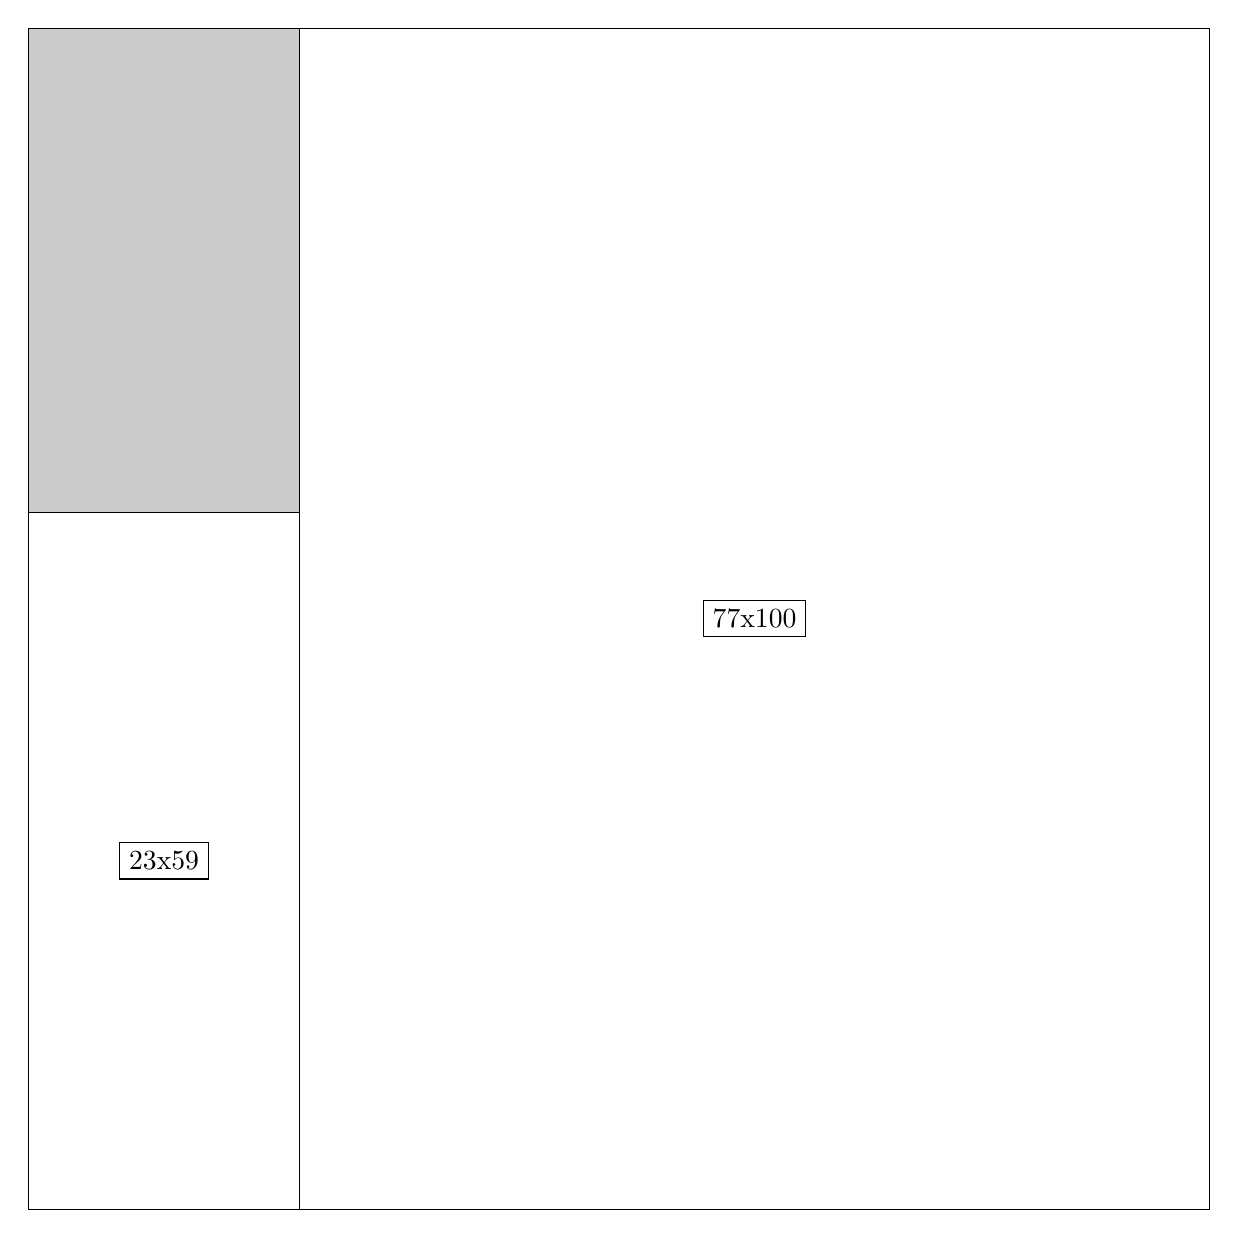
\begin{tikzpicture}[shorten >=1pt,scale=1.0,every node/.style={scale=1.0},->]
\tikzstyle{vertex}=[circle,fill=black!25,minimum size=14pt,inner sep=0pt]
\filldraw[fill=gray!40!white, draw=black] (0,0) rectangle (15.0,15.0);
\foreach \name/\x/\y/\w/\h in {77x100/3.4499999999999997/0.0/11.549999999999999/15.0,23x59/0.0/0.0/3.4499999999999997/8.85}
\filldraw[fill=white!40!white, draw=black] (\x,\y) rectangle node[draw] (\name) {\name} ++(\w,\h);
\end{tikzpicture}


w =77 , h =100 , x =23 , y =0 , v =7700
\par
w =23 , h =59 , x =0 , y =0 , v =1357
\par
\newpage


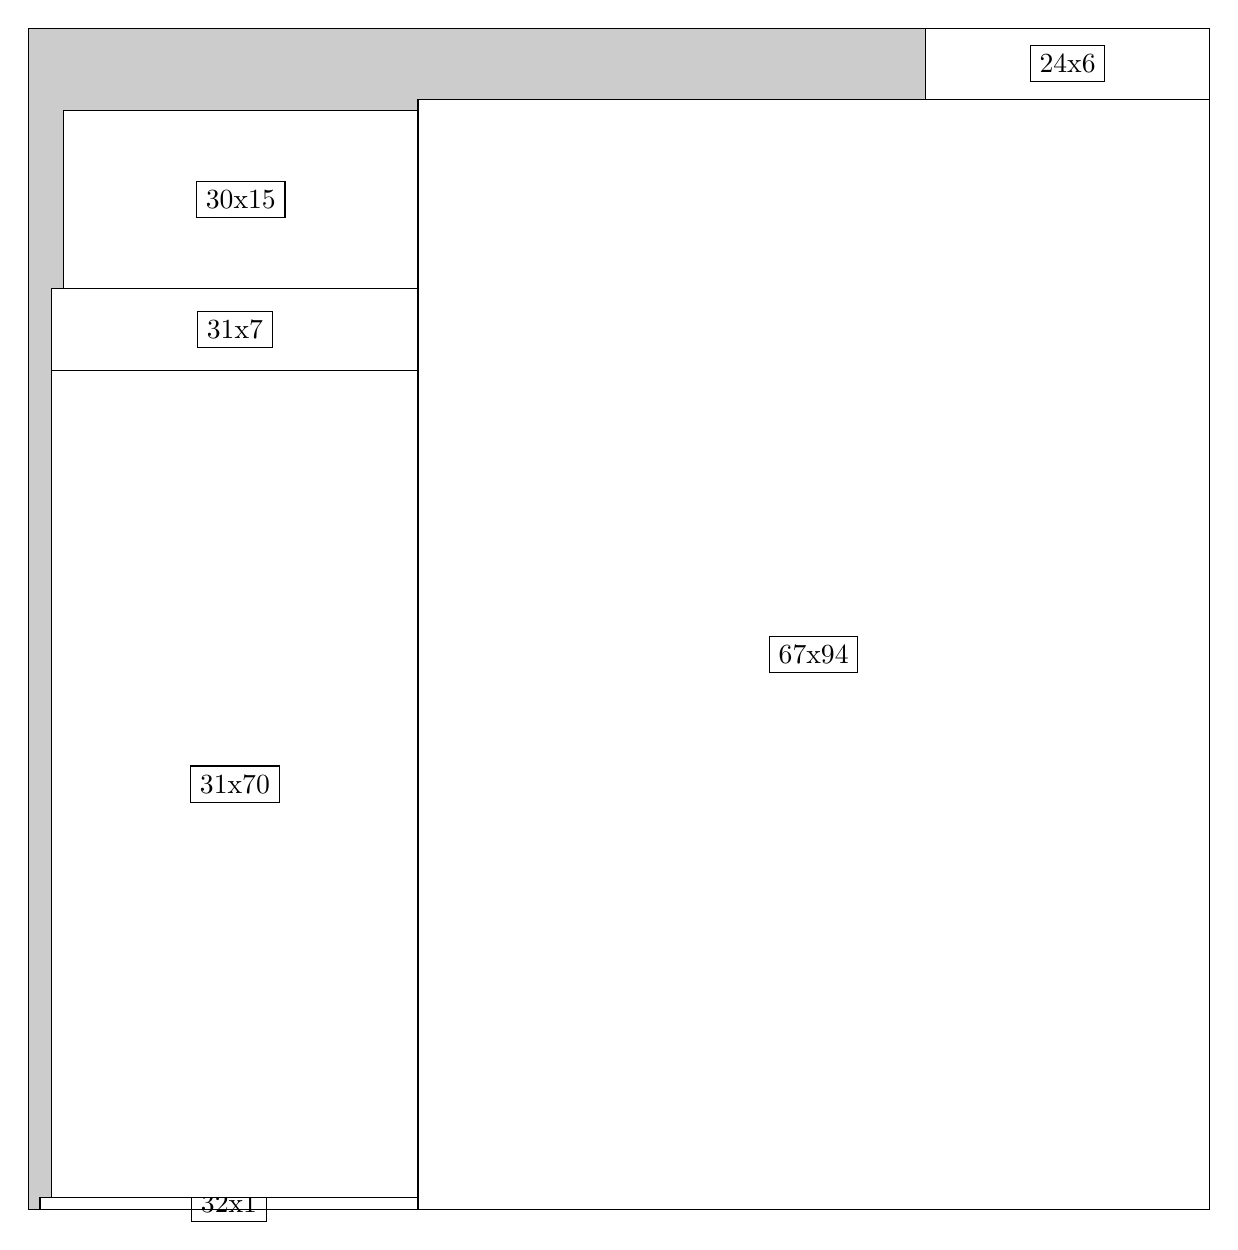
\begin{tikzpicture}[shorten >=1pt,scale=1.0,every node/.style={scale=1.0},->]
\tikzstyle{vertex}=[circle,fill=black!25,minimum size=14pt,inner sep=0pt]
\filldraw[fill=gray!40!white, draw=black] (0,0) rectangle (15.0,15.0);
\foreach \name/\x/\y/\w/\h in {67x94/4.95/0.0/10.049999999999999/14.1,32x1/0.15/0.0/4.8/0.15,31x70/0.3/0.15/4.6499999999999995/10.5,31x7/0.3/10.65/4.6499999999999995/1.05,30x15/0.44999999999999996/11.7/4.5/2.25,24x6/11.4/14.1/3.5999999999999996/0.8999999999999999}
\filldraw[fill=white!40!white, draw=black] (\x,\y) rectangle node[draw] (\name) {\name} ++(\w,\h);
\end{tikzpicture}


w =67 , h =94 , x =33 , y =0 , v =6298
\par
w =32 , h =1 , x =1 , y =0 , v =32
\par
w =31 , h =70 , x =2 , y =1 , v =2170
\par
w =31 , h =7 , x =2 , y =71 , v =217
\par
w =30 , h =15 , x =3 , y =78 , v =450
\par
w =24 , h =6 , x =76 , y =94 , v =144
\par
\newpage


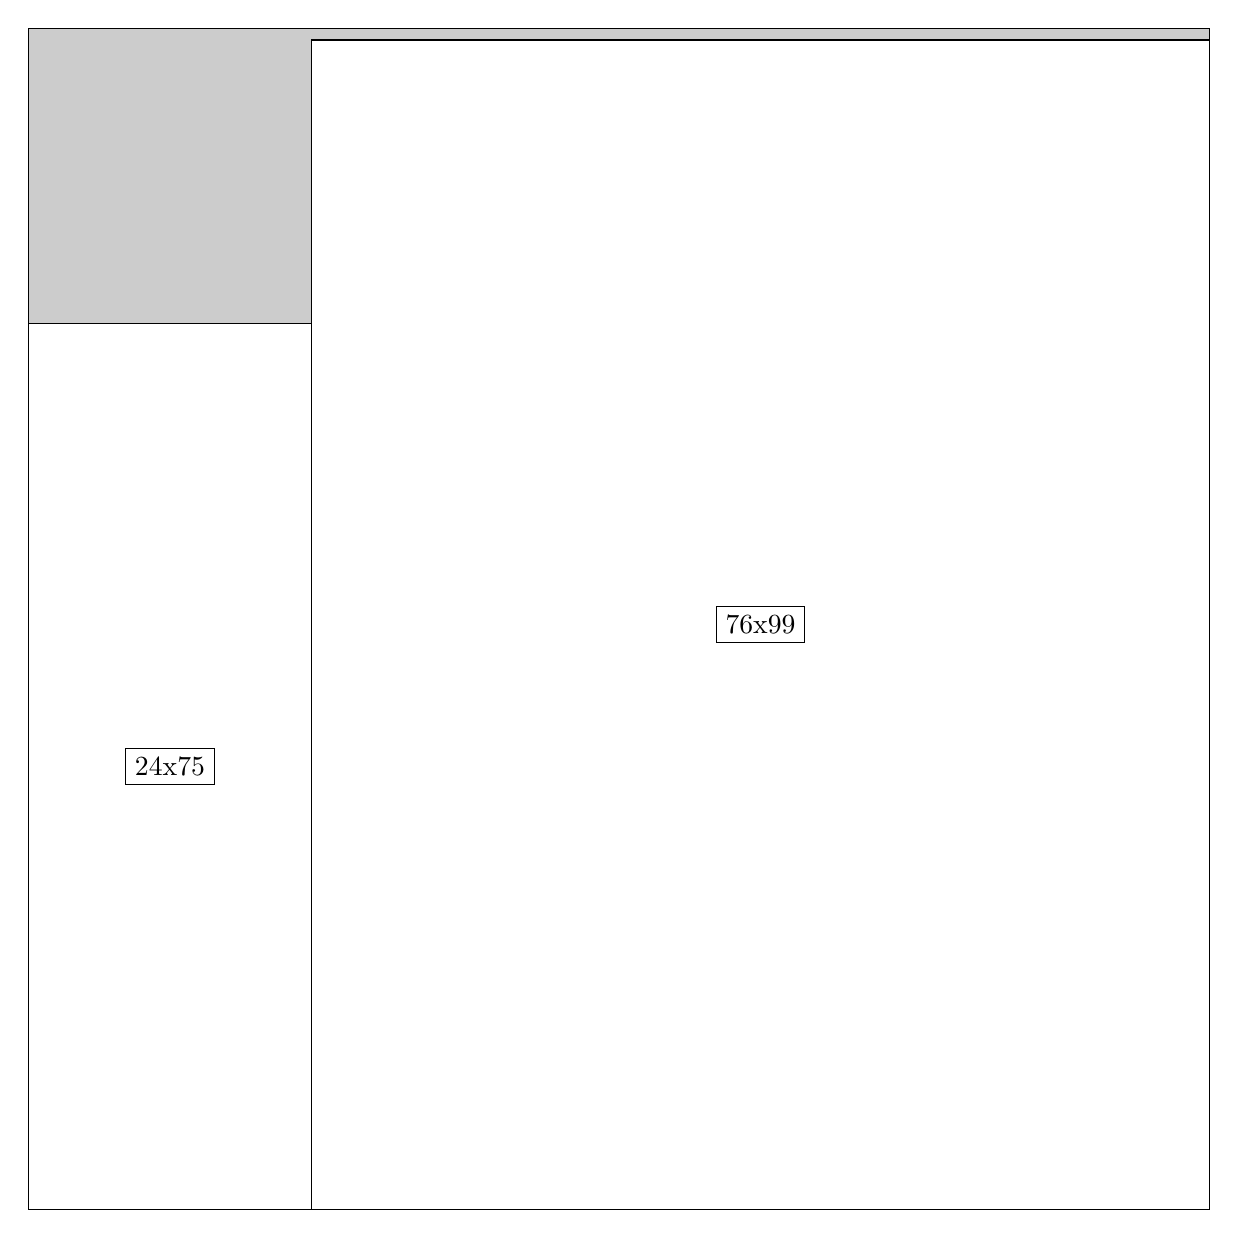
\begin{tikzpicture}[shorten >=1pt,scale=1.0,every node/.style={scale=1.0},->]
\tikzstyle{vertex}=[circle,fill=black!25,minimum size=14pt,inner sep=0pt]
\filldraw[fill=gray!40!white, draw=black] (0,0) rectangle (15.0,15.0);
\foreach \name/\x/\y/\w/\h in {76x99/3.5999999999999996/0.0/11.4/14.85,24x75/0.0/0.0/3.5999999999999996/11.25}
\filldraw[fill=white!40!white, draw=black] (\x,\y) rectangle node[draw] (\name) {\name} ++(\w,\h);
\end{tikzpicture}


w =76 , h =99 , x =24 , y =0 , v =7524
\par
w =24 , h =75 , x =0 , y =0 , v =1800
\par
\newpage


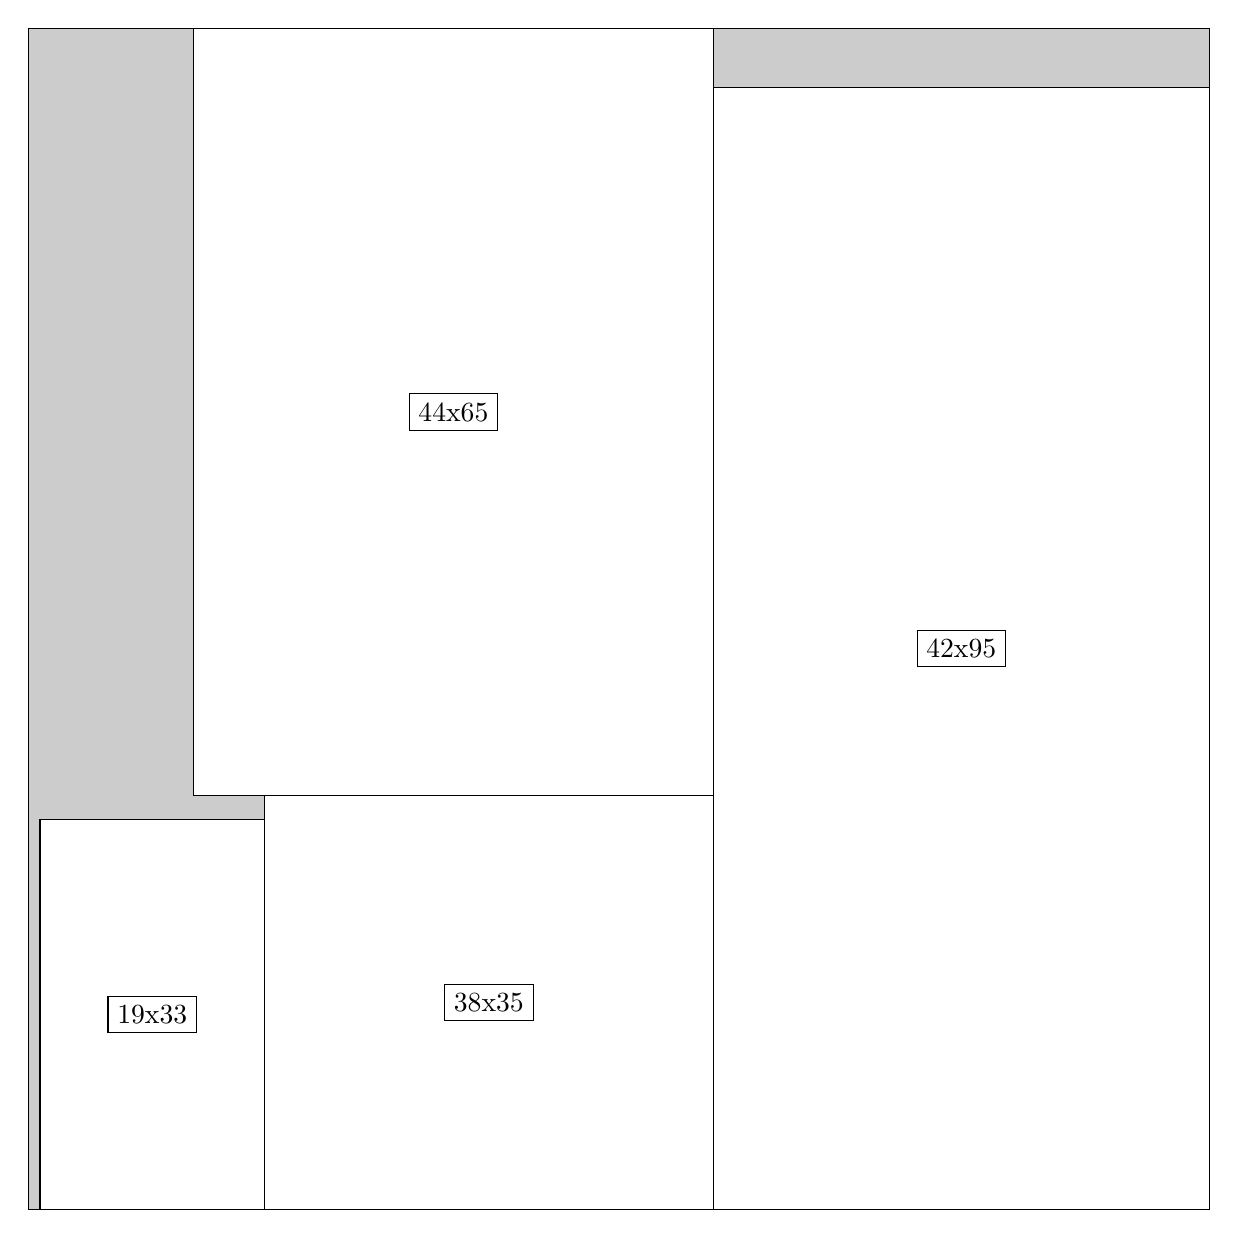
\begin{tikzpicture}[shorten >=1pt,scale=1.0,every node/.style={scale=1.0},->]
\tikzstyle{vertex}=[circle,fill=black!25,minimum size=14pt,inner sep=0pt]
\filldraw[fill=gray!40!white, draw=black] (0,0) rectangle (15.0,15.0);
\foreach \name/\x/\y/\w/\h in {42x95/8.7/0.0/6.3/14.25,38x35/3.0/0.0/5.7/5.25,19x33/0.15/0.0/2.85/4.95,44x65/2.1/5.25/6.6/9.75}
\filldraw[fill=white!40!white, draw=black] (\x,\y) rectangle node[draw] (\name) {\name} ++(\w,\h);
\end{tikzpicture}


w =42 , h =95 , x =58 , y =0 , v =3990
\par
w =38 , h =35 , x =20 , y =0 , v =1330
\par
w =19 , h =33 , x =1 , y =0 , v =627
\par
w =44 , h =65 , x =14 , y =35 , v =2860
\par
\newpage


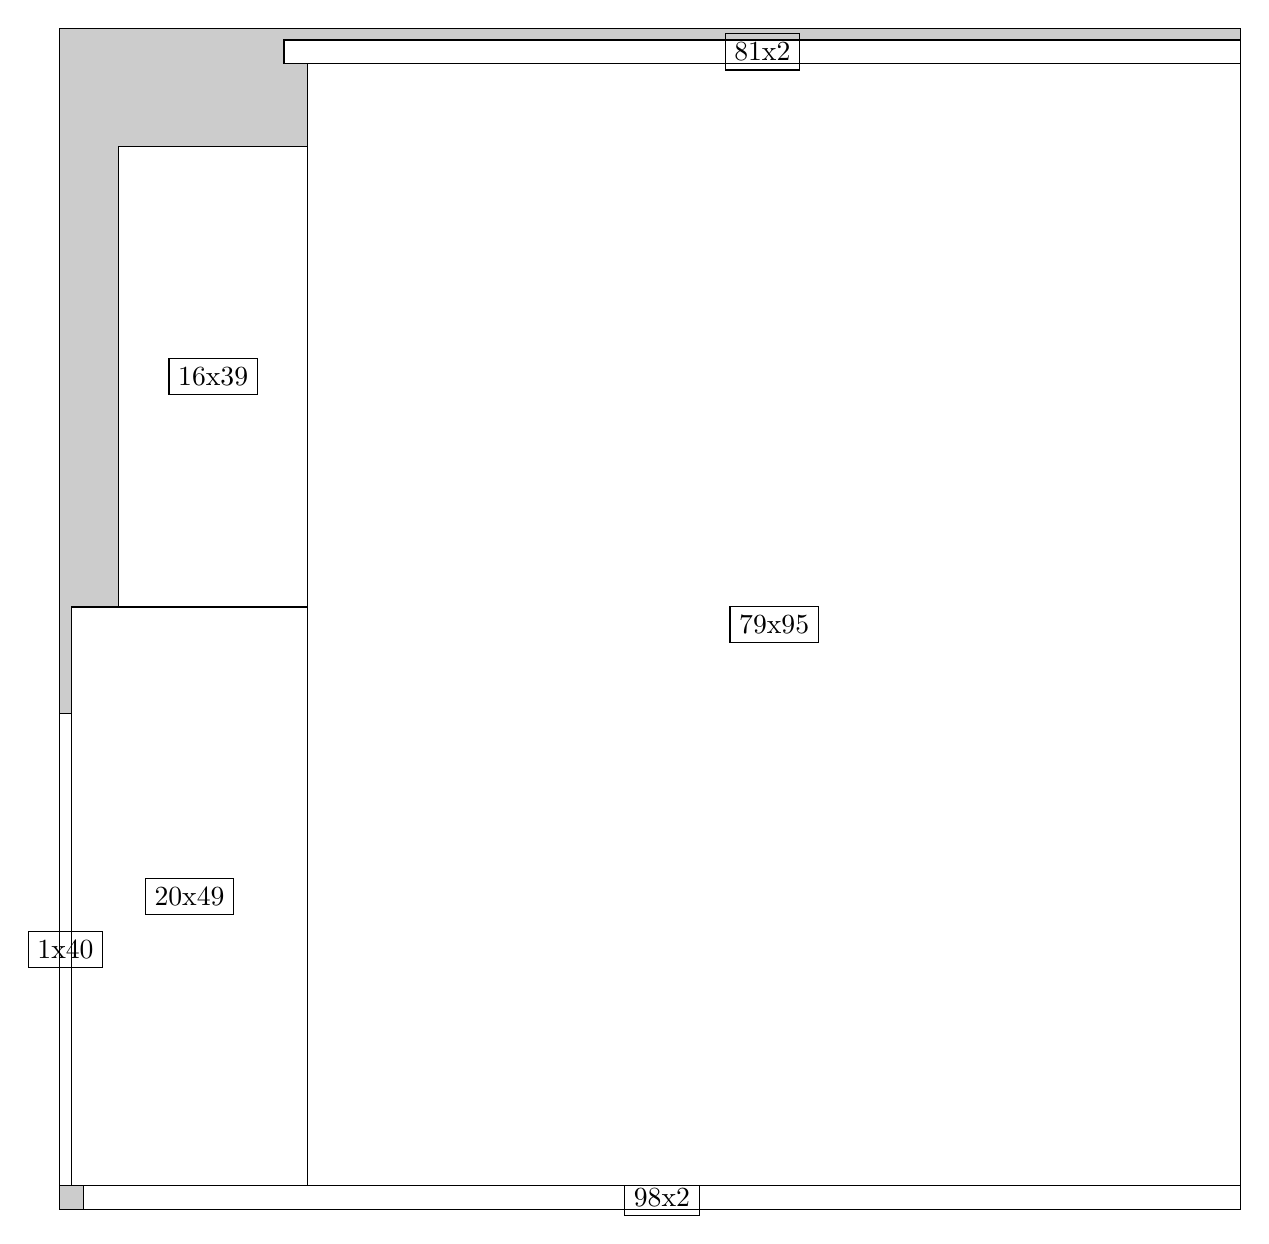
\begin{tikzpicture}[shorten >=1pt,scale=1.0,every node/.style={scale=1.0},->]
\tikzstyle{vertex}=[circle,fill=black!25,minimum size=14pt,inner sep=0pt]
\filldraw[fill=gray!40!white, draw=black] (0,0) rectangle (15.0,15.0);
\foreach \name/\x/\y/\w/\h in {98x2/0.3/0.0/14.7/0.3,79x95/3.15/0.3/11.85/14.25,20x49/0.15/0.3/3.0/7.35,1x40/0.0/0.3/0.15/6.0,16x39/0.75/7.6499999999999995/2.4/5.85,81x2/2.85/14.549999999999999/12.15/0.3}
\filldraw[fill=white!40!white, draw=black] (\x,\y) rectangle node[draw] (\name) {\name} ++(\w,\h);
\end{tikzpicture}


w =98 , h =2 , x =2 , y =0 , v =196
\par
w =79 , h =95 , x =21 , y =2 , v =7505
\par
w =20 , h =49 , x =1 , y =2 , v =980
\par
w =1 , h =40 , x =0 , y =2 , v =40
\par
w =16 , h =39 , x =5 , y =51 , v =624
\par
w =81 , h =2 , x =19 , y =97 , v =162
\par
\newpage


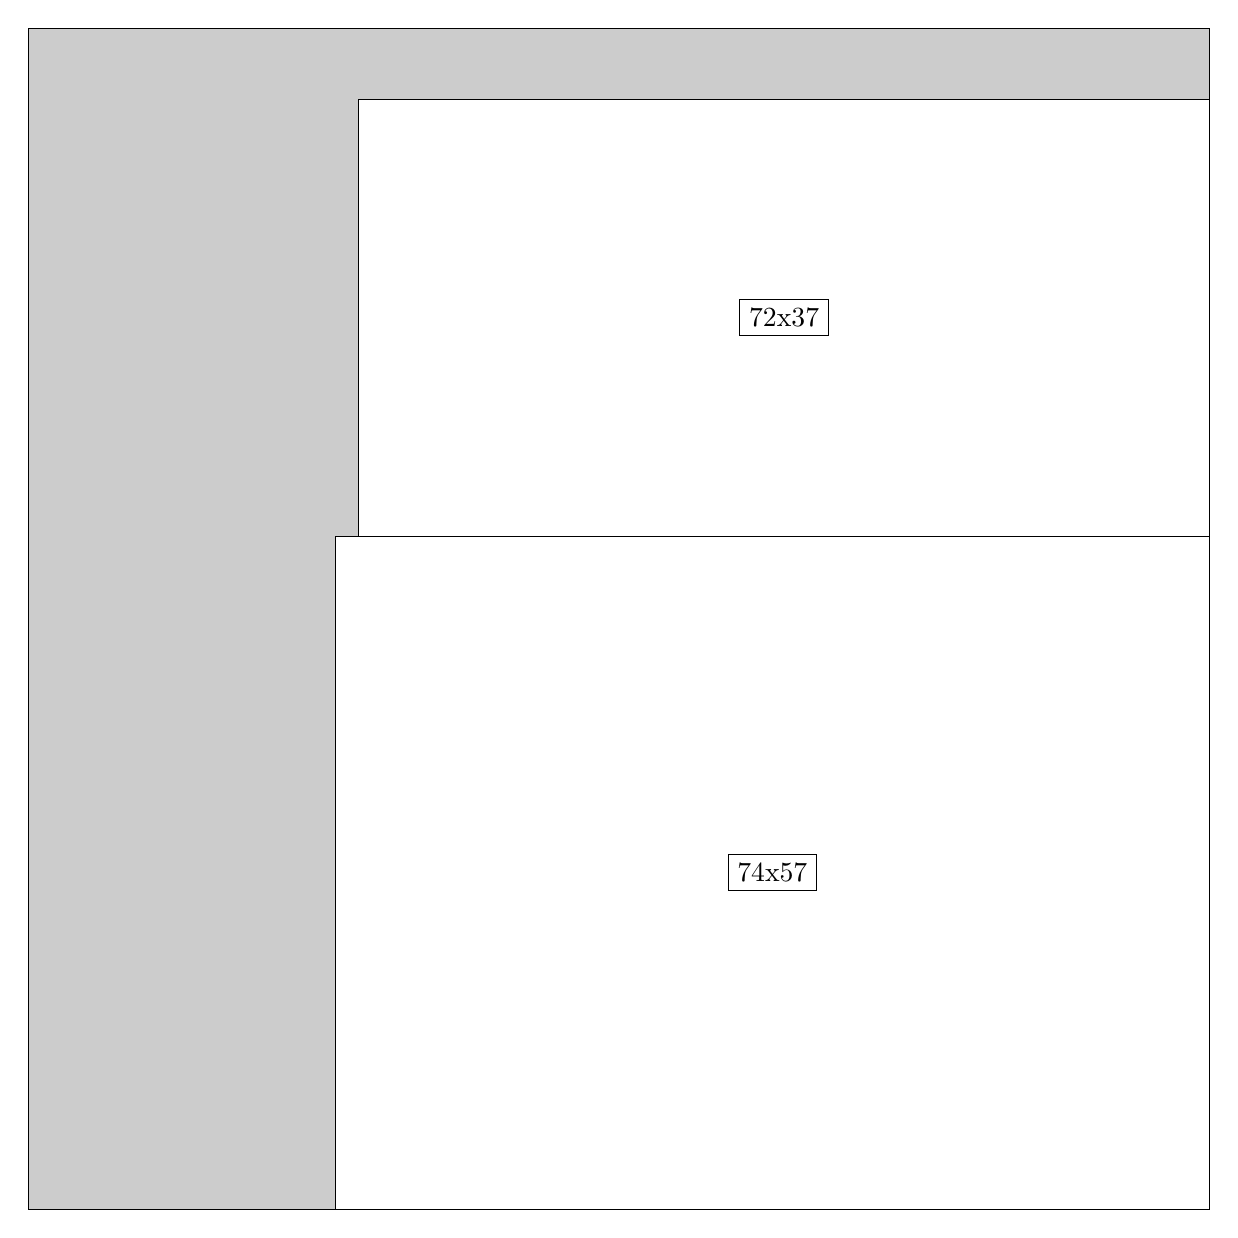
\begin{tikzpicture}[shorten >=1pt,scale=1.0,every node/.style={scale=1.0},->]
\tikzstyle{vertex}=[circle,fill=black!25,minimum size=14pt,inner sep=0pt]
\filldraw[fill=gray!40!white, draw=black] (0,0) rectangle (15.0,15.0);
\foreach \name/\x/\y/\w/\h in {74x57/3.9/0.0/11.1/8.549999999999999,72x37/4.2/8.549999999999999/10.799999999999999/5.55}
\filldraw[fill=white!40!white, draw=black] (\x,\y) rectangle node[draw] (\name) {\name} ++(\w,\h);
\end{tikzpicture}


w =74 , h =57 , x =26 , y =0 , v =4218
\par
w =72 , h =37 , x =28 , y =57 , v =2664
\par
\newpage


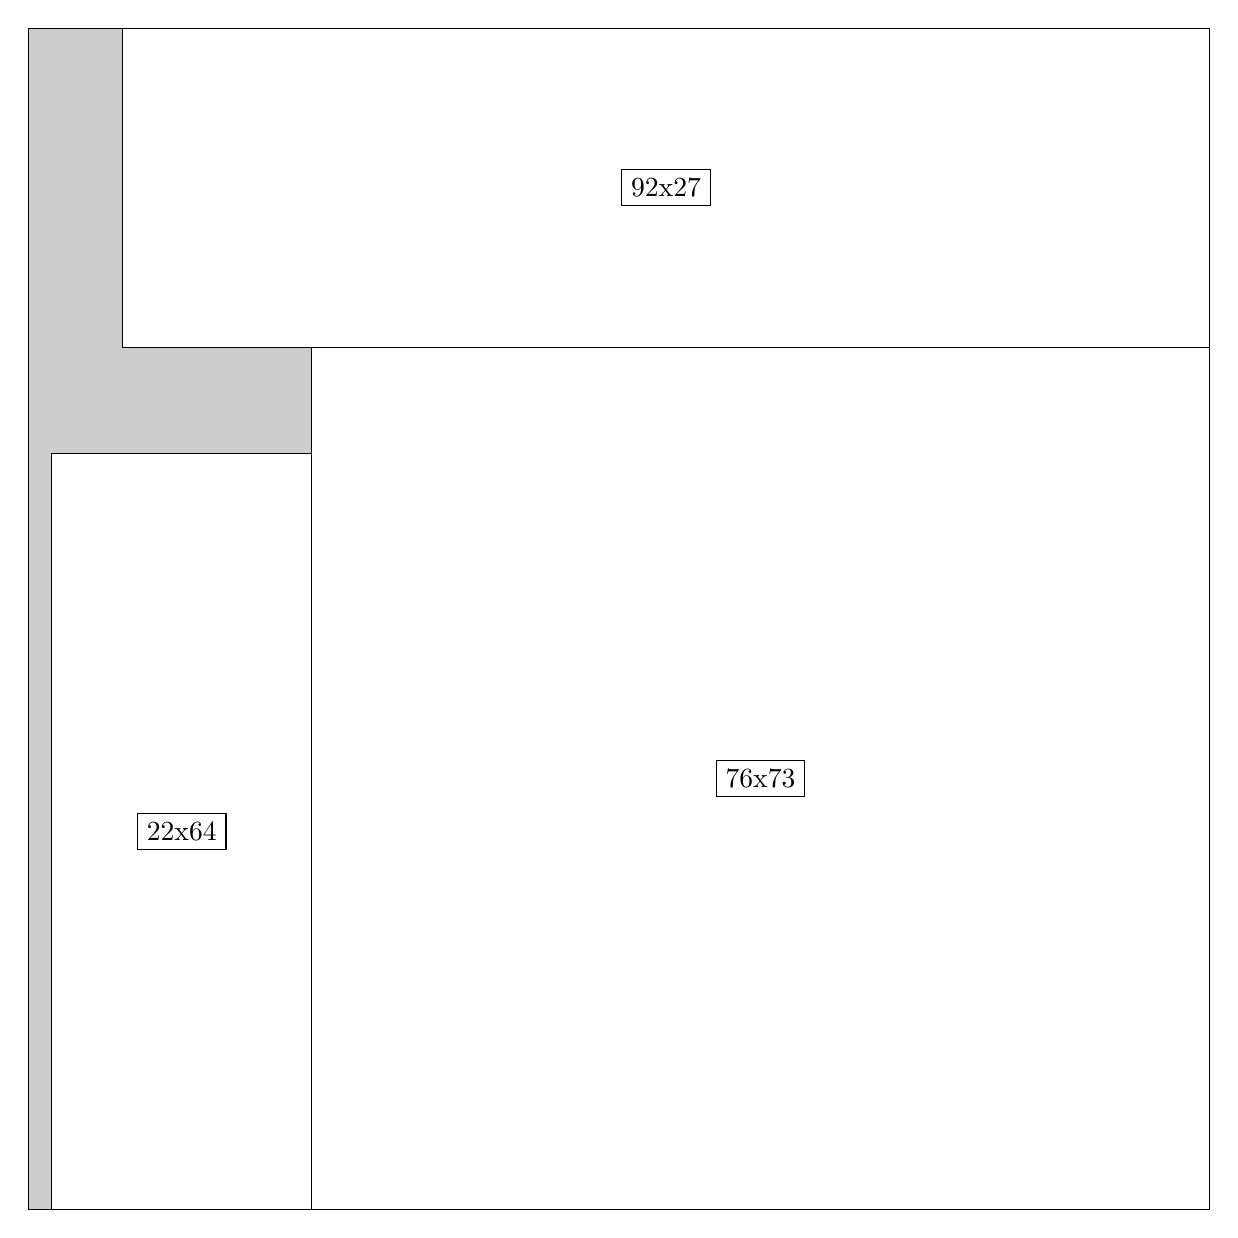
\begin{tikzpicture}[shorten >=1pt,scale=1.0,every node/.style={scale=1.0},->]
\tikzstyle{vertex}=[circle,fill=black!25,minimum size=14pt,inner sep=0pt]
\filldraw[fill=gray!40!white, draw=black] (0,0) rectangle (15.0,15.0);
\foreach \name/\x/\y/\w/\h in {76x73/3.5999999999999996/0.0/11.4/10.95,22x64/0.3/0.0/3.3/9.6,92x27/1.2/10.95/13.799999999999999/4.05}
\filldraw[fill=white!40!white, draw=black] (\x,\y) rectangle node[draw] (\name) {\name} ++(\w,\h);
\end{tikzpicture}


w =76 , h =73 , x =24 , y =0 , v =5548
\par
w =22 , h =64 , x =2 , y =0 , v =1408
\par
w =92 , h =27 , x =8 , y =73 , v =2484
\par
\newpage


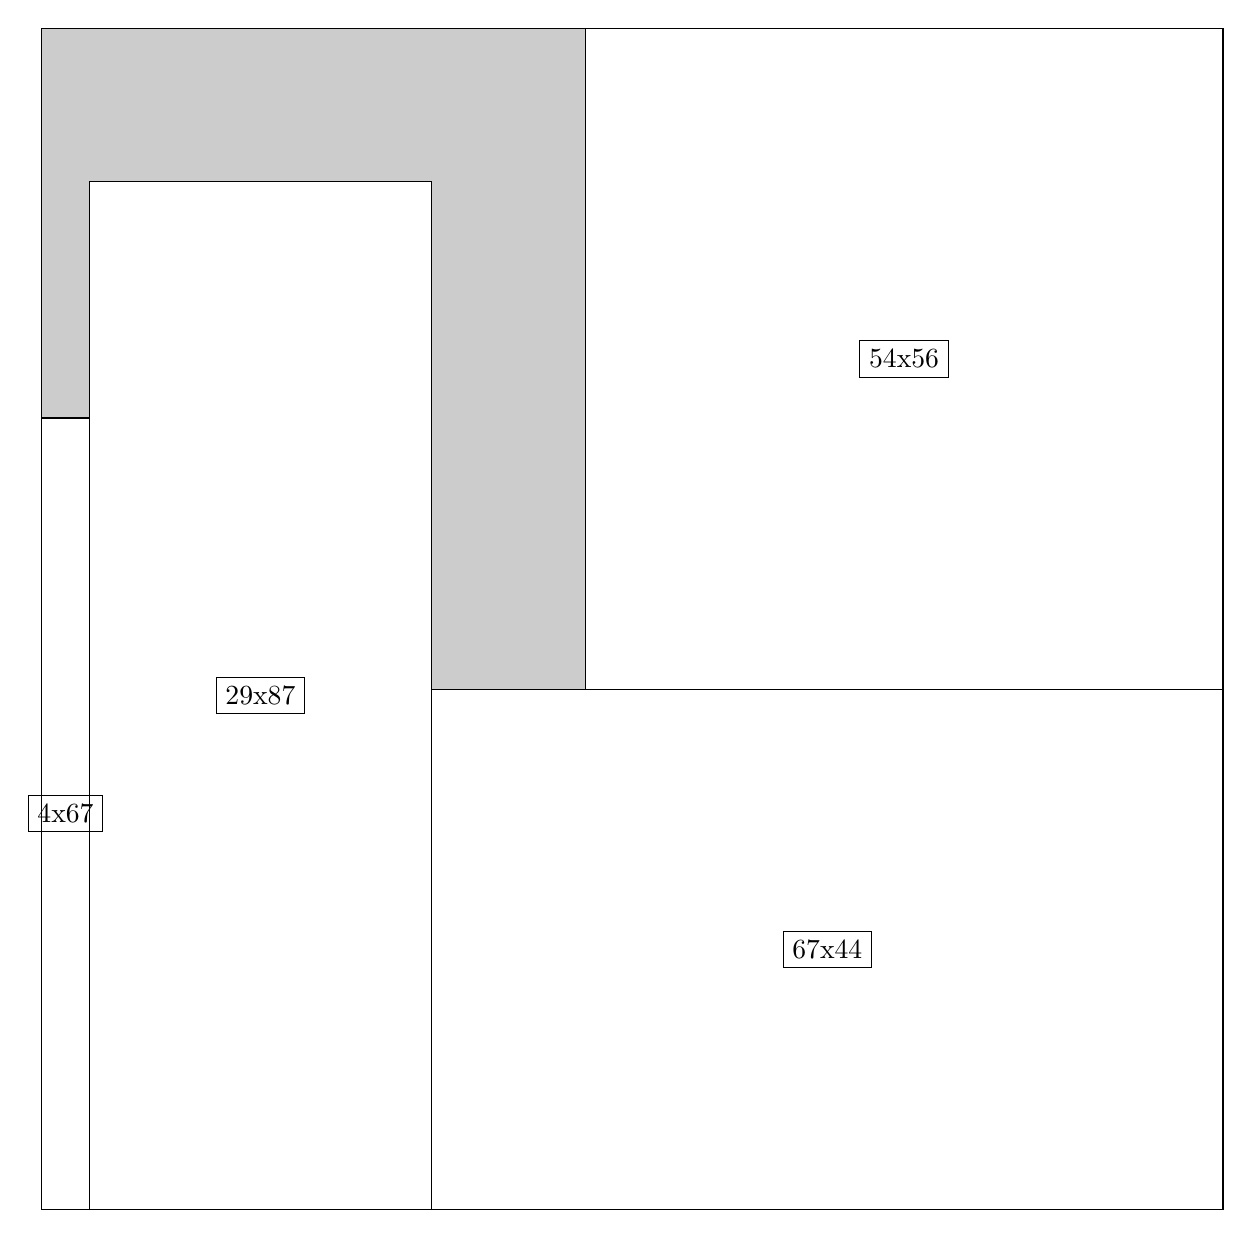
\begin{tikzpicture}[shorten >=1pt,scale=1.0,every node/.style={scale=1.0},->]
\tikzstyle{vertex}=[circle,fill=black!25,minimum size=14pt,inner sep=0pt]
\filldraw[fill=gray!40!white, draw=black] (0,0) rectangle (15.0,15.0);
\foreach \name/\x/\y/\w/\h in {67x44/4.95/0.0/10.049999999999999/6.6,54x56/6.8999999999999995/6.6/8.1/8.4,29x87/0.6/0.0/4.35/13.049999999999999,4x67/0.0/0.0/0.6/10.049999999999999}
\filldraw[fill=white!40!white, draw=black] (\x,\y) rectangle node[draw] (\name) {\name} ++(\w,\h);
\end{tikzpicture}


w =67 , h =44 , x =33 , y =0 , v =2948
\par
w =54 , h =56 , x =46 , y =44 , v =3024
\par
w =29 , h =87 , x =4 , y =0 , v =2523
\par
w =4 , h =67 , x =0 , y =0 , v =268
\par
\newpage


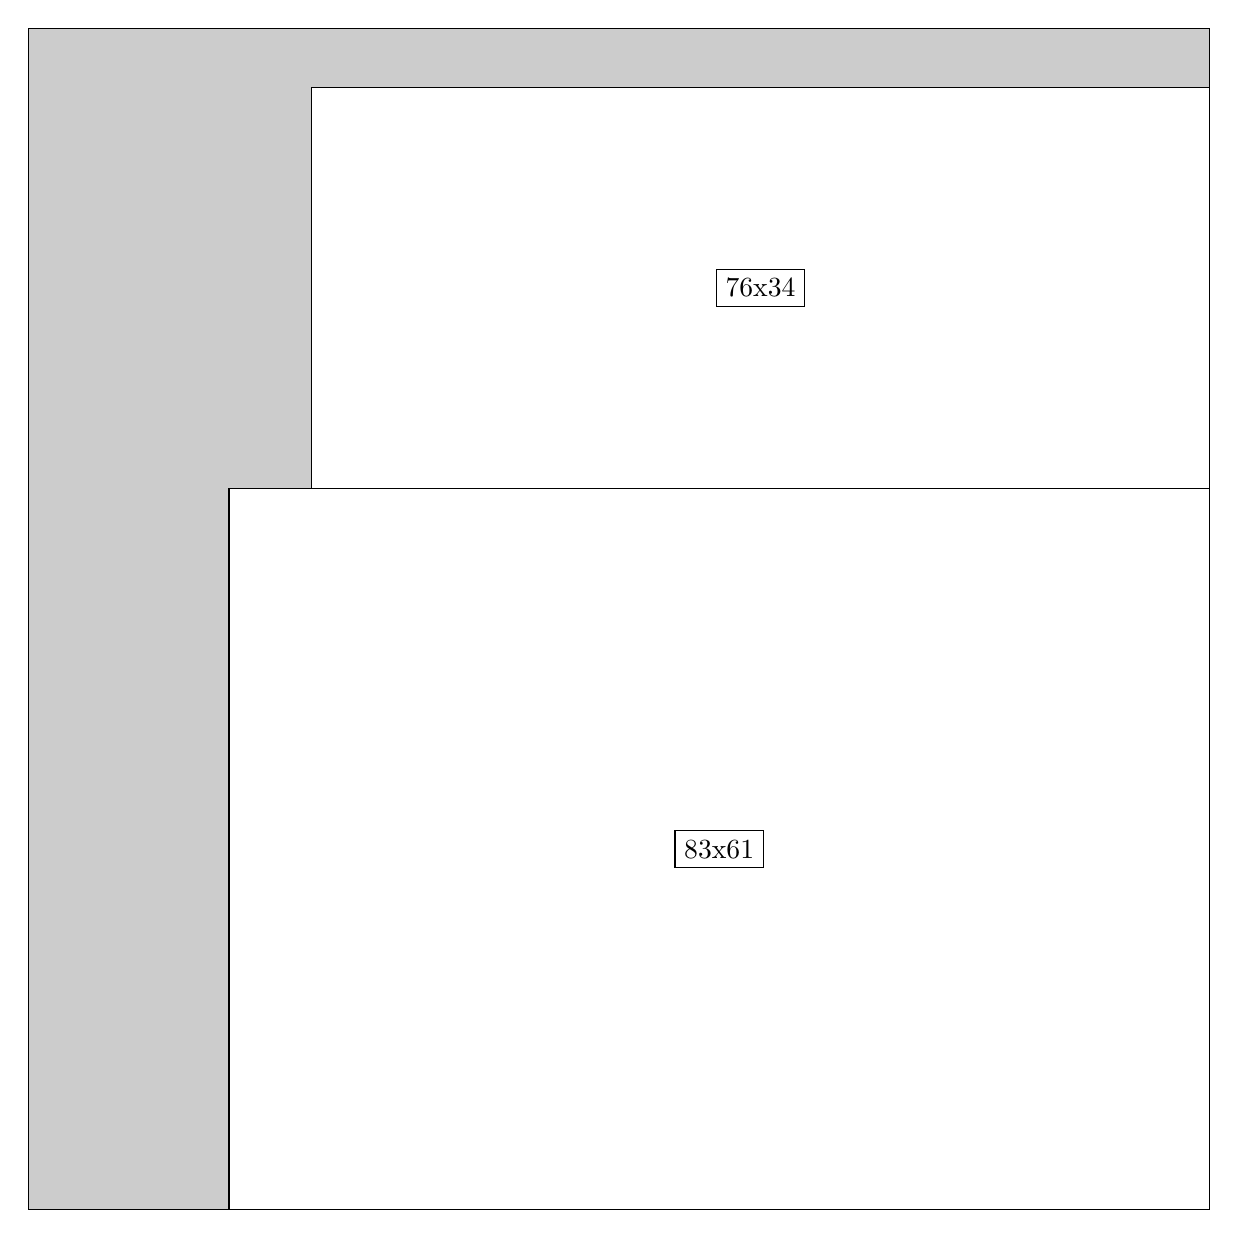
\begin{tikzpicture}[shorten >=1pt,scale=1.0,every node/.style={scale=1.0},->]
\tikzstyle{vertex}=[circle,fill=black!25,minimum size=14pt,inner sep=0pt]
\filldraw[fill=gray!40!white, draw=black] (0,0) rectangle (15.0,15.0);
\foreach \name/\x/\y/\w/\h in {83x61/2.55/0.0/12.45/9.15,76x34/3.5999999999999996/9.15/11.4/5.1}
\filldraw[fill=white!40!white, draw=black] (\x,\y) rectangle node[draw] (\name) {\name} ++(\w,\h);
\end{tikzpicture}


w =83 , h =61 , x =17 , y =0 , v =5063
\par
w =76 , h =34 , x =24 , y =61 , v =2584
\par
\newpage


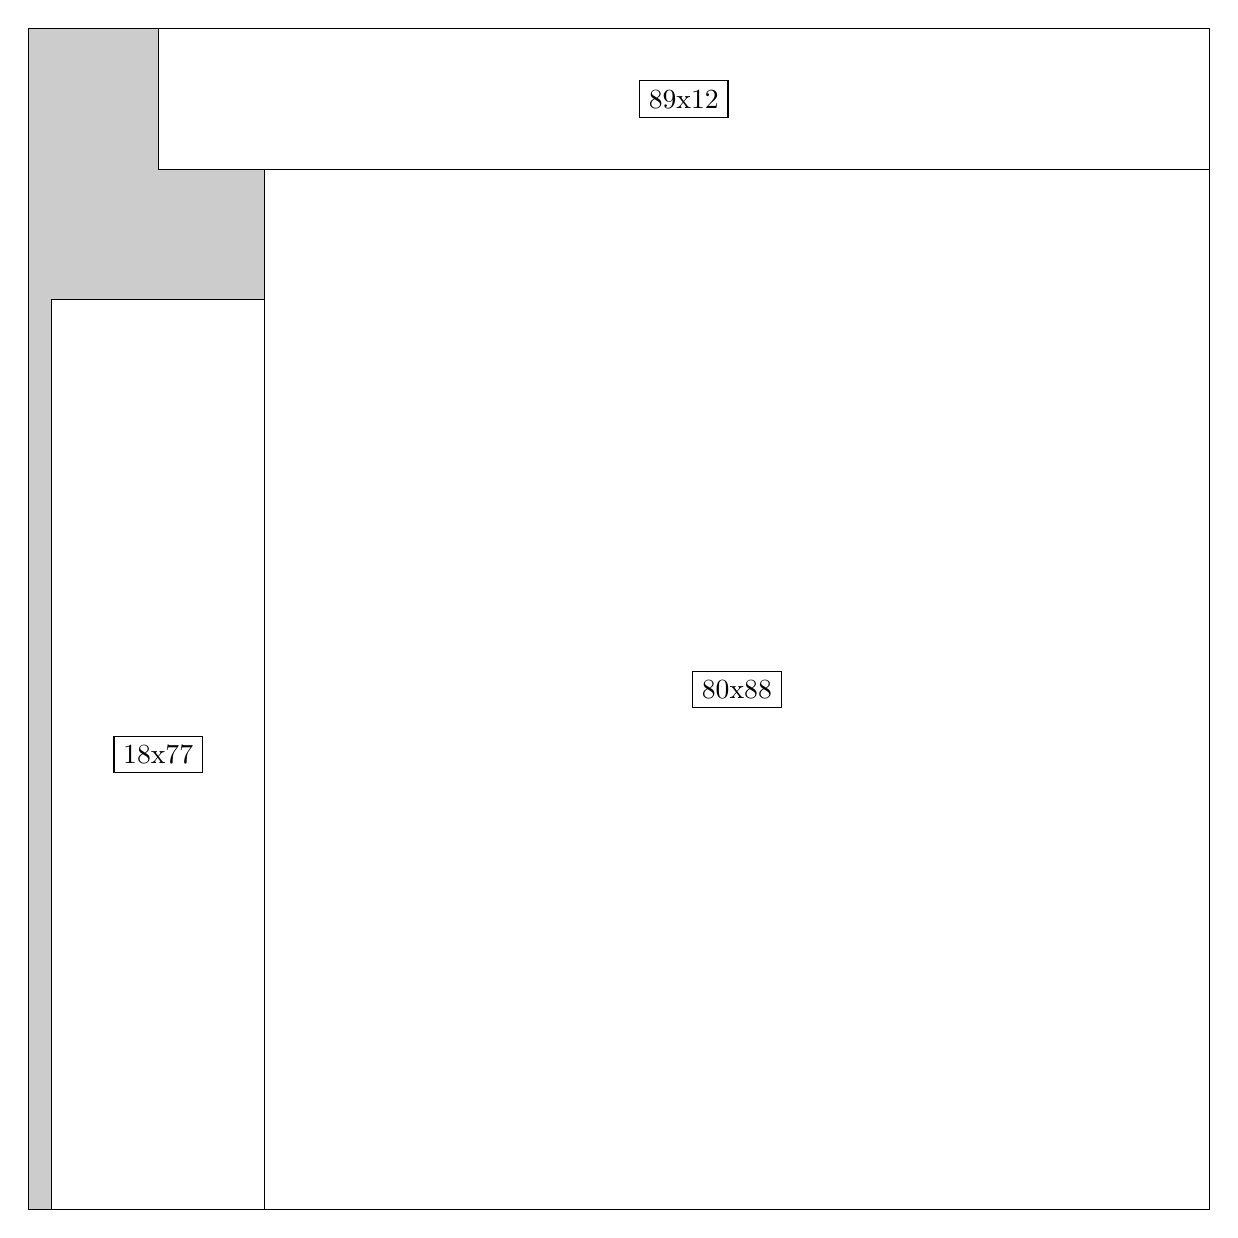
\begin{tikzpicture}[shorten >=1pt,scale=1.0,every node/.style={scale=1.0},->]
\tikzstyle{vertex}=[circle,fill=black!25,minimum size=14pt,inner sep=0pt]
\filldraw[fill=gray!40!white, draw=black] (0,0) rectangle (15.0,15.0);
\foreach \name/\x/\y/\w/\h in {80x88/3.0/0.0/12.0/13.2,18x77/0.3/0.0/2.6999999999999997/11.549999999999999,89x12/1.65/13.2/13.35/1.7999999999999998}
\filldraw[fill=white!40!white, draw=black] (\x,\y) rectangle node[draw] (\name) {\name} ++(\w,\h);
\end{tikzpicture}


w =80 , h =88 , x =20 , y =0 , v =7040
\par
w =18 , h =77 , x =2 , y =0 , v =1386
\par
w =89 , h =12 , x =11 , y =88 , v =1068
\par
\newpage


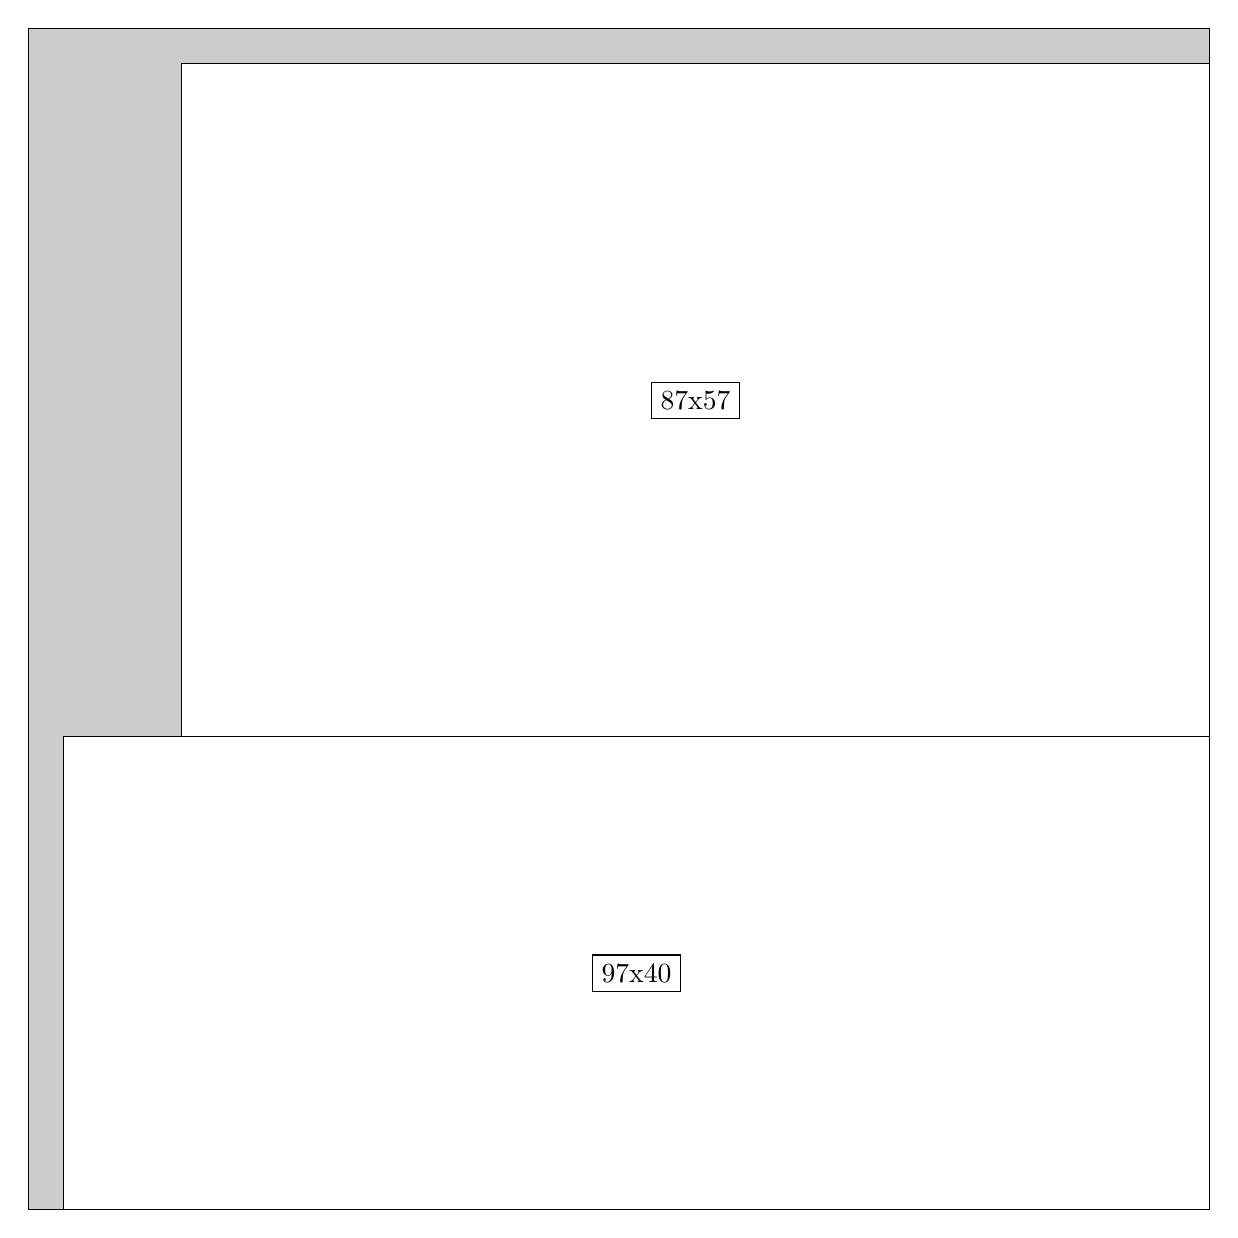
\begin{tikzpicture}[shorten >=1pt,scale=1.0,every node/.style={scale=1.0},->]
\tikzstyle{vertex}=[circle,fill=black!25,minimum size=14pt,inner sep=0pt]
\filldraw[fill=gray!40!white, draw=black] (0,0) rectangle (15.0,15.0);
\foreach \name/\x/\y/\w/\h in {97x40/0.44999999999999996/0.0/14.549999999999999/6.0,87x57/1.95/6.0/13.049999999999999/8.549999999999999}
\filldraw[fill=white!40!white, draw=black] (\x,\y) rectangle node[draw] (\name) {\name} ++(\w,\h);
\end{tikzpicture}


w =97 , h =40 , x =3 , y =0 , v =3880
\par
w =87 , h =57 , x =13 , y =40 , v =4959
\par
\newpage


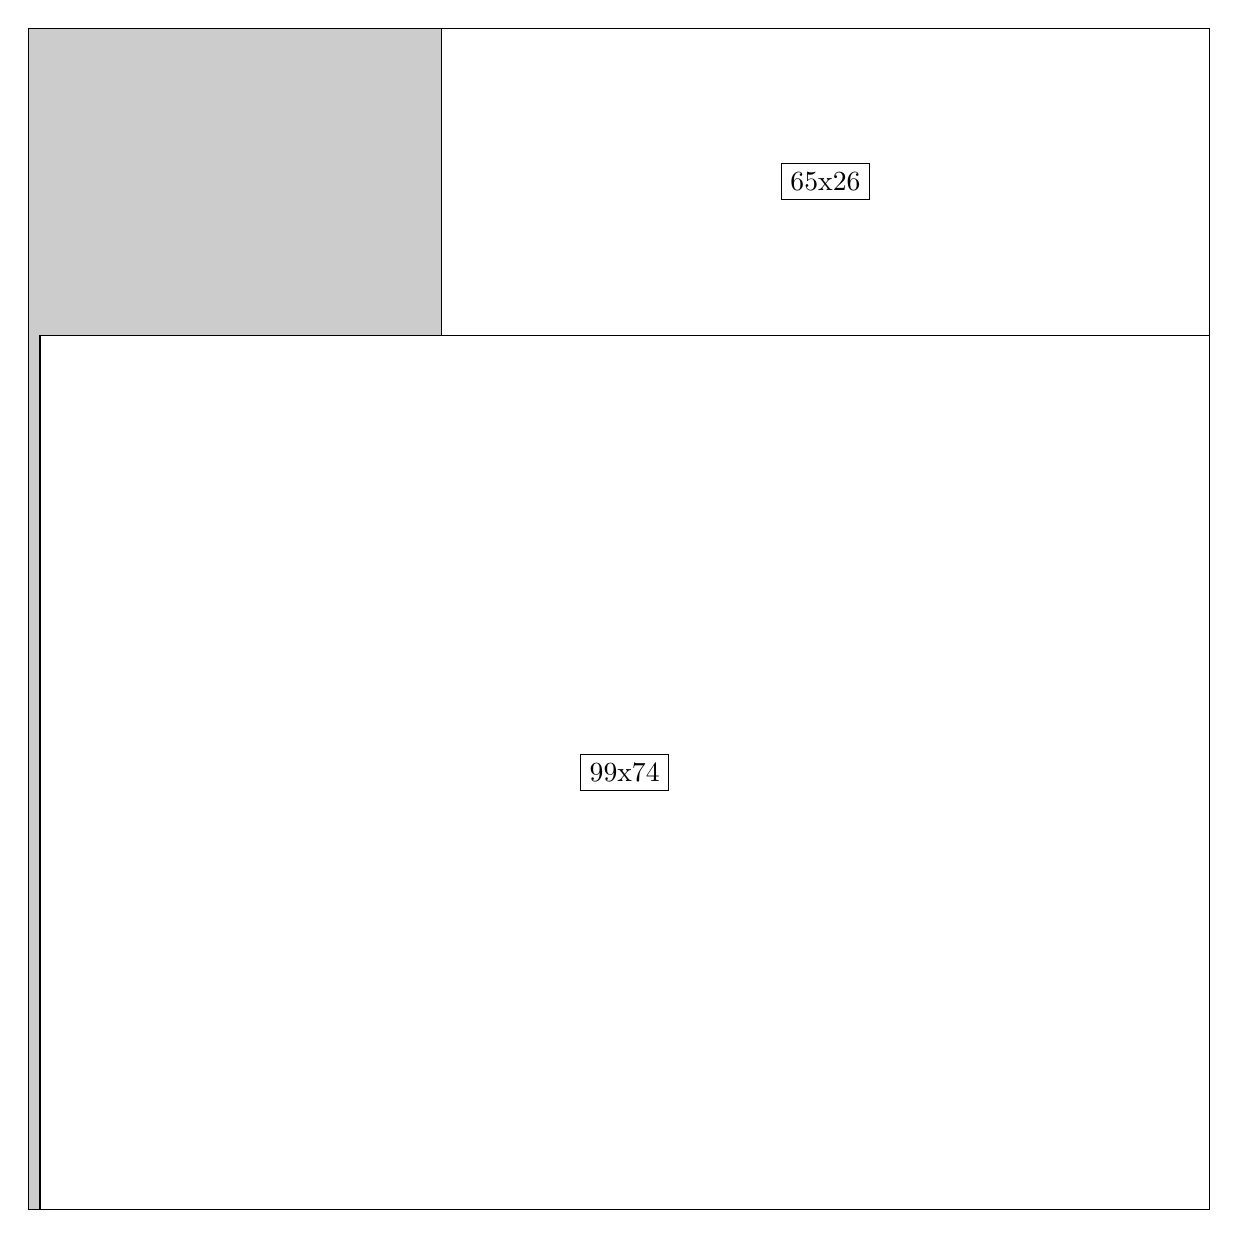
\begin{tikzpicture}[shorten >=1pt,scale=1.0,every node/.style={scale=1.0},->]
\tikzstyle{vertex}=[circle,fill=black!25,minimum size=14pt,inner sep=0pt]
\filldraw[fill=gray!40!white, draw=black] (0,0) rectangle (15.0,15.0);
\foreach \name/\x/\y/\w/\h in {99x74/0.15/0.0/14.85/11.1,65x26/5.25/11.1/9.75/3.9}
\filldraw[fill=white!40!white, draw=black] (\x,\y) rectangle node[draw] (\name) {\name} ++(\w,\h);
\end{tikzpicture}


w =99 , h =74 , x =1 , y =0 , v =7326
\par
w =65 , h =26 , x =35 , y =74 , v =1690
\par
\newpage


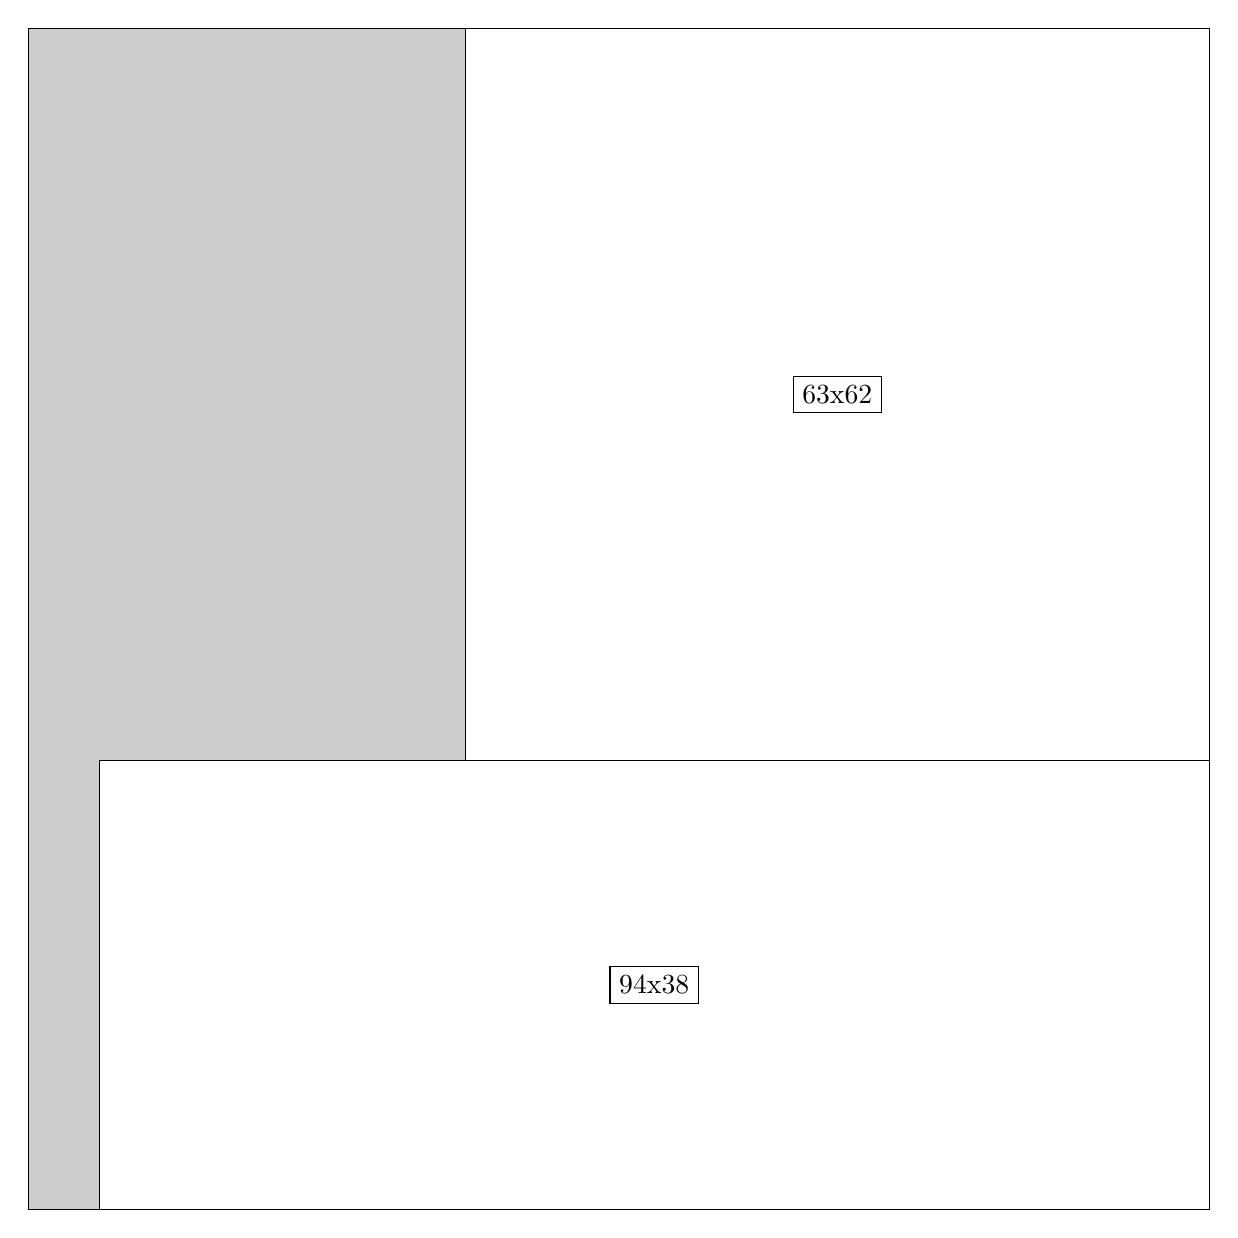
\begin{tikzpicture}[shorten >=1pt,scale=1.0,every node/.style={scale=1.0},->]
\tikzstyle{vertex}=[circle,fill=black!25,minimum size=14pt,inner sep=0pt]
\filldraw[fill=gray!40!white, draw=black] (0,0) rectangle (15.0,15.0);
\foreach \name/\x/\y/\w/\h in {94x38/0.8999999999999999/0.0/14.1/5.7,63x62/5.55/5.7/9.45/9.299999999999999}
\filldraw[fill=white!40!white, draw=black] (\x,\y) rectangle node[draw] (\name) {\name} ++(\w,\h);
\end{tikzpicture}


w =94 , h =38 , x =6 , y =0 , v =3572
\par
w =63 , h =62 , x =37 , y =38 , v =3906
\par
\newpage


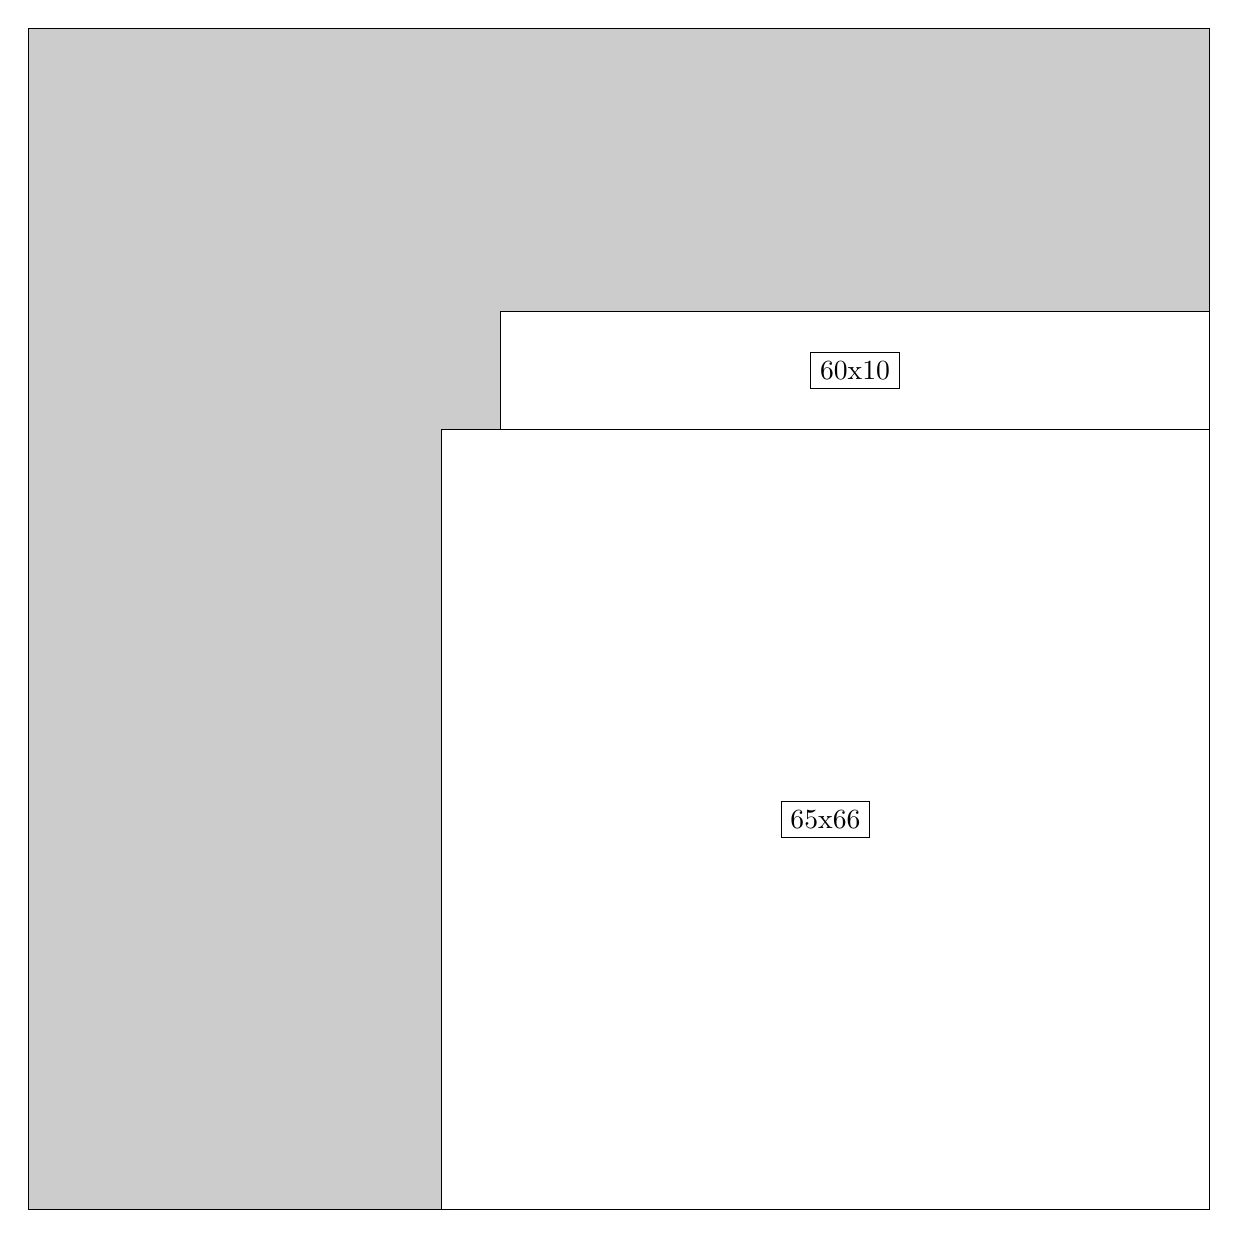
\begin{tikzpicture}[shorten >=1pt,scale=1.0,every node/.style={scale=1.0},->]
\tikzstyle{vertex}=[circle,fill=black!25,minimum size=14pt,inner sep=0pt]
\filldraw[fill=gray!40!white, draw=black] (0,0) rectangle (15.0,15.0);
\foreach \name/\x/\y/\w/\h in {65x66/5.25/0.0/9.75/9.9,60x10/6.0/9.9/9.0/1.5}
\filldraw[fill=white!40!white, draw=black] (\x,\y) rectangle node[draw] (\name) {\name} ++(\w,\h);
\end{tikzpicture}


w =65 , h =66 , x =35 , y =0 , v =4290
\par
w =60 , h =10 , x =40 , y =66 , v =600
\par
\newpage


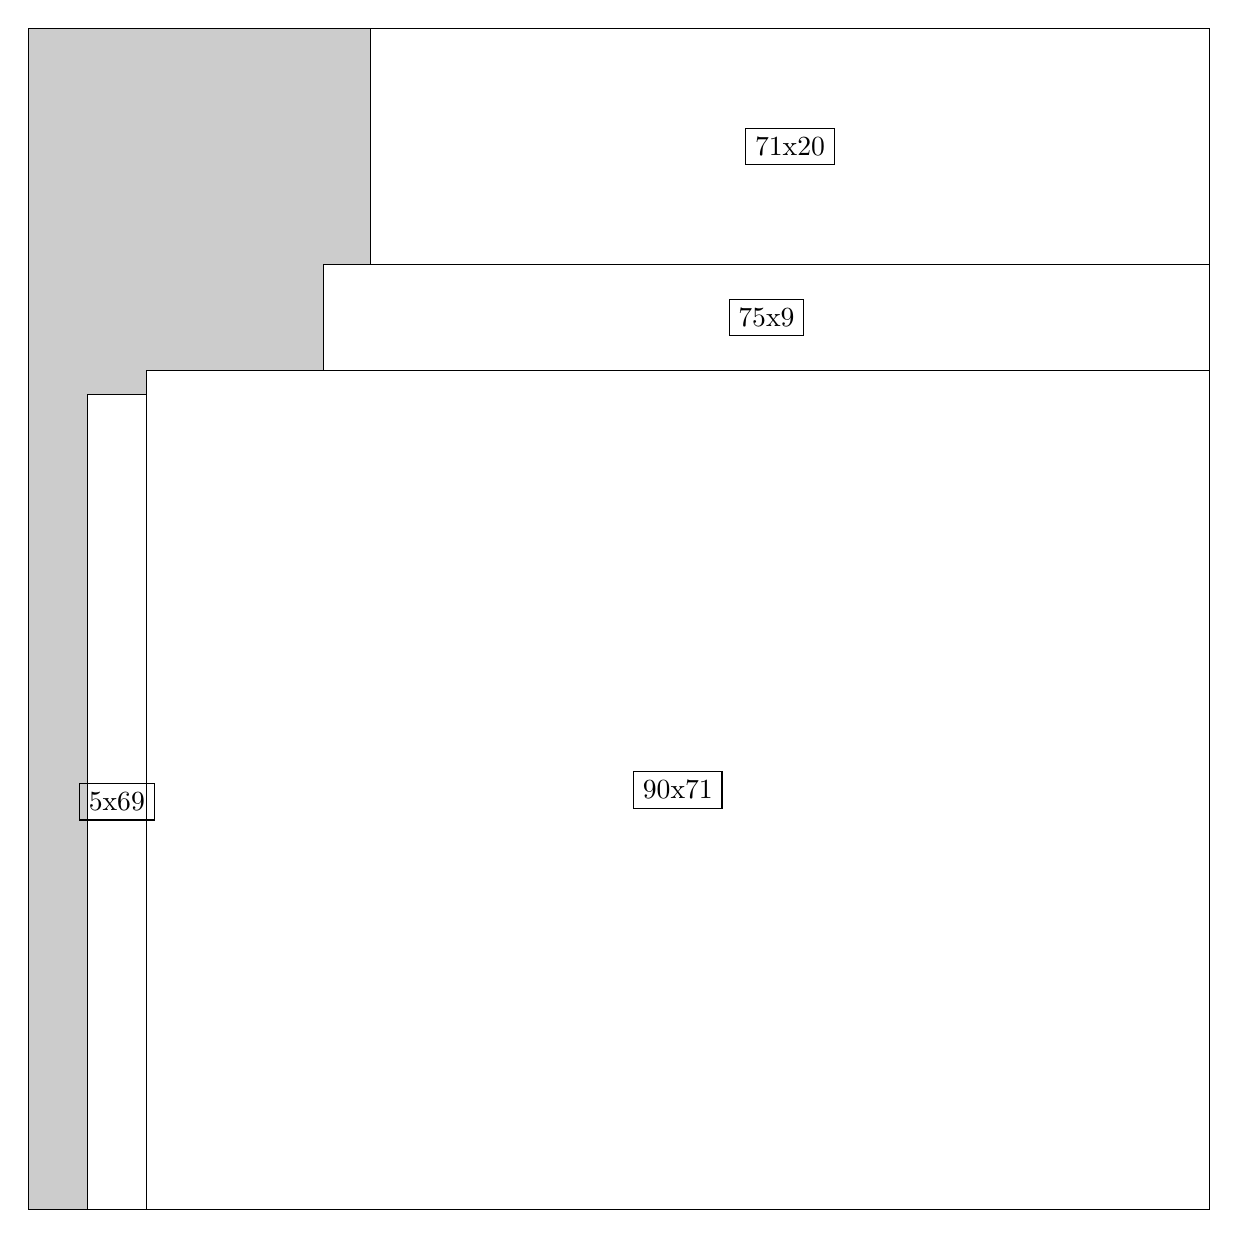
\begin{tikzpicture}[shorten >=1pt,scale=1.0,every node/.style={scale=1.0},->]
\tikzstyle{vertex}=[circle,fill=black!25,minimum size=14pt,inner sep=0pt]
\filldraw[fill=gray!40!white, draw=black] (0,0) rectangle (15.0,15.0);
\foreach \name/\x/\y/\w/\h in {90x71/1.5/0.0/13.5/10.65,75x9/3.75/10.65/11.25/1.3499999999999999,71x20/4.35/12.0/10.65/3.0,5x69/0.75/0.0/0.75/10.35}
\filldraw[fill=white!40!white, draw=black] (\x,\y) rectangle node[draw] (\name) {\name} ++(\w,\h);
\end{tikzpicture}


w =90 , h =71 , x =10 , y =0 , v =6390
\par
w =75 , h =9 , x =25 , y =71 , v =675
\par
w =71 , h =20 , x =29 , y =80 , v =1420
\par
w =5 , h =69 , x =5 , y =0 , v =345
\par
\newpage


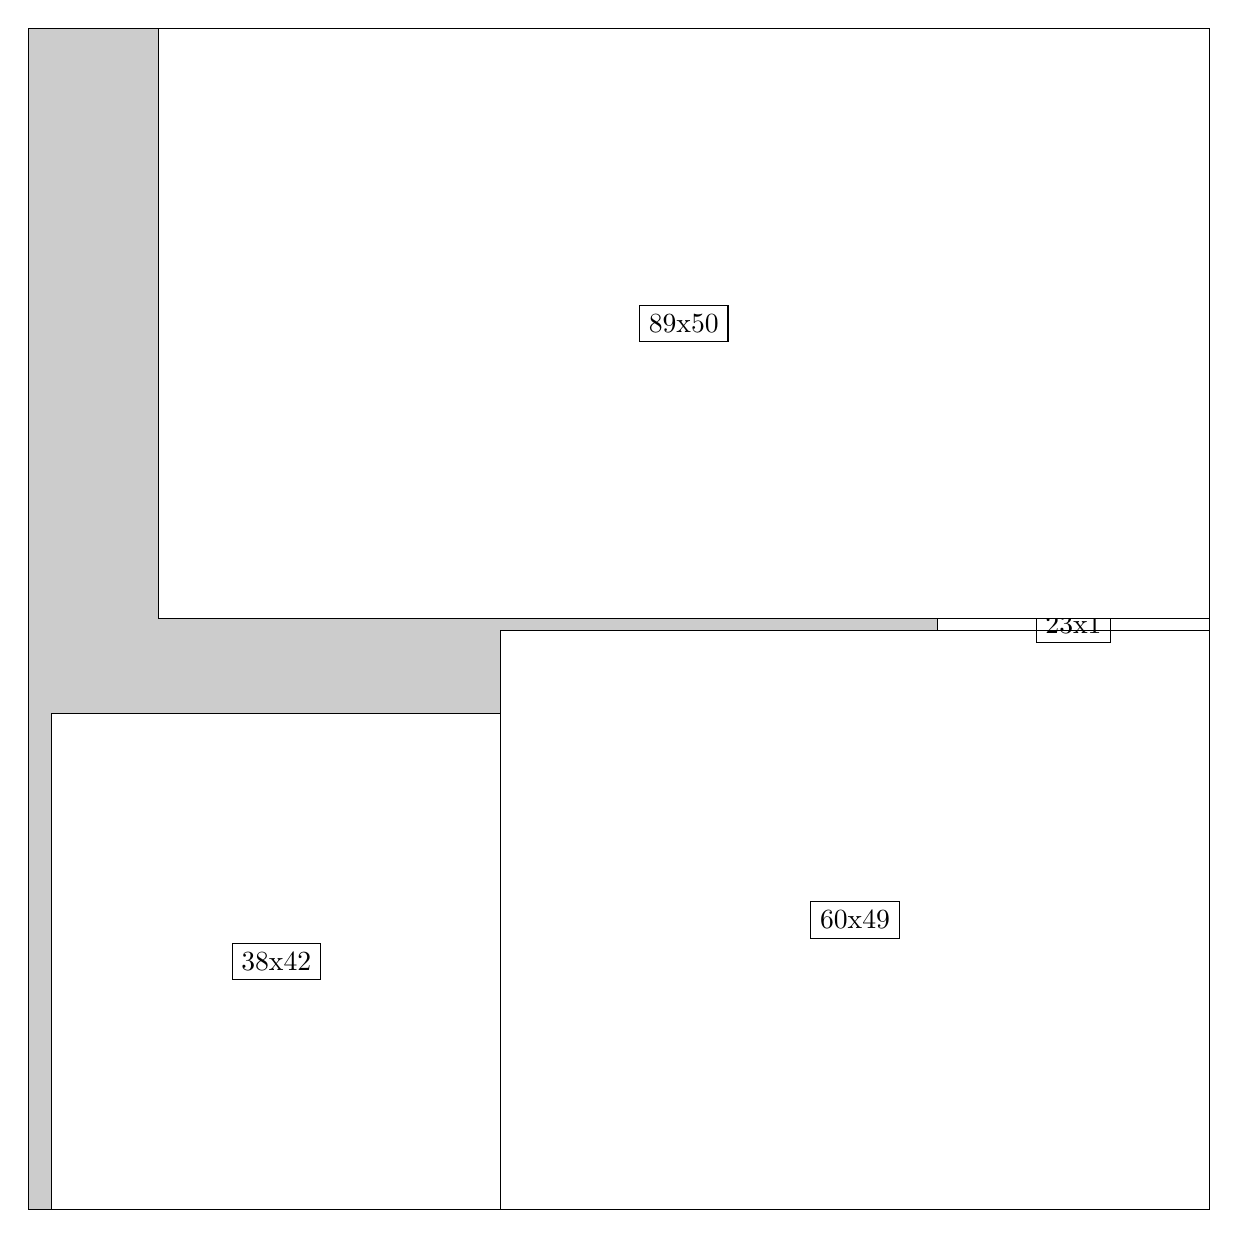
\begin{tikzpicture}[shorten >=1pt,scale=1.0,every node/.style={scale=1.0},->]
\tikzstyle{vertex}=[circle,fill=black!25,minimum size=14pt,inner sep=0pt]
\filldraw[fill=gray!40!white, draw=black] (0,0) rectangle (15.0,15.0);
\foreach \name/\x/\y/\w/\h in {60x49/6.0/0.0/9.0/7.35,23x1/11.549999999999999/7.35/3.4499999999999997/0.15,38x42/0.3/0.0/5.7/6.3,89x50/1.65/7.5/13.35/7.5}
\filldraw[fill=white!40!white, draw=black] (\x,\y) rectangle node[draw] (\name) {\name} ++(\w,\h);
\end{tikzpicture}


w =60 , h =49 , x =40 , y =0 , v =2940
\par
w =23 , h =1 , x =77 , y =49 , v =23
\par
w =38 , h =42 , x =2 , y =0 , v =1596
\par
w =89 , h =50 , x =11 , y =50 , v =4450
\par
\newpage


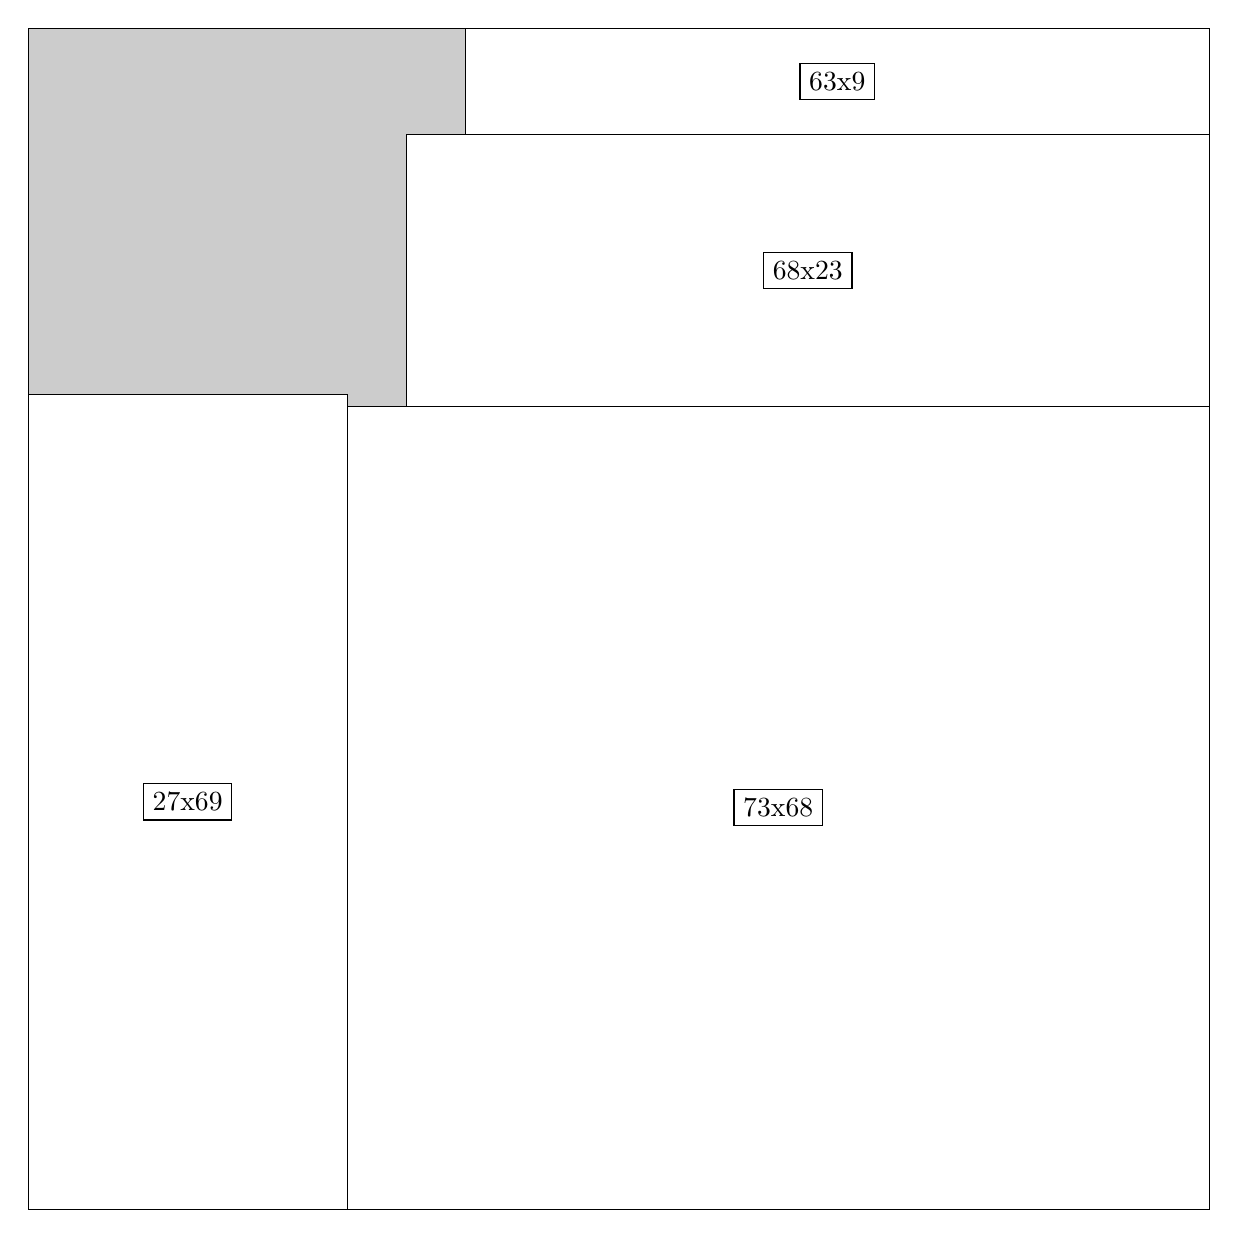
\begin{tikzpicture}[shorten >=1pt,scale=1.0,every node/.style={scale=1.0},->]
\tikzstyle{vertex}=[circle,fill=black!25,minimum size=14pt,inner sep=0pt]
\filldraw[fill=gray!40!white, draw=black] (0,0) rectangle (15.0,15.0);
\foreach \name/\x/\y/\w/\h in {73x68/4.05/0.0/10.95/10.2,68x23/4.8/10.2/10.2/3.4499999999999997,63x9/5.55/13.65/9.45/1.3499999999999999,27x69/0.0/0.0/4.05/10.35}
\filldraw[fill=white!40!white, draw=black] (\x,\y) rectangle node[draw] (\name) {\name} ++(\w,\h);
\end{tikzpicture}


w =73 , h =68 , x =27 , y =0 , v =4964
\par
w =68 , h =23 , x =32 , y =68 , v =1564
\par
w =63 , h =9 , x =37 , y =91 , v =567
\par
w =27 , h =69 , x =0 , y =0 , v =1863
\par
\newpage


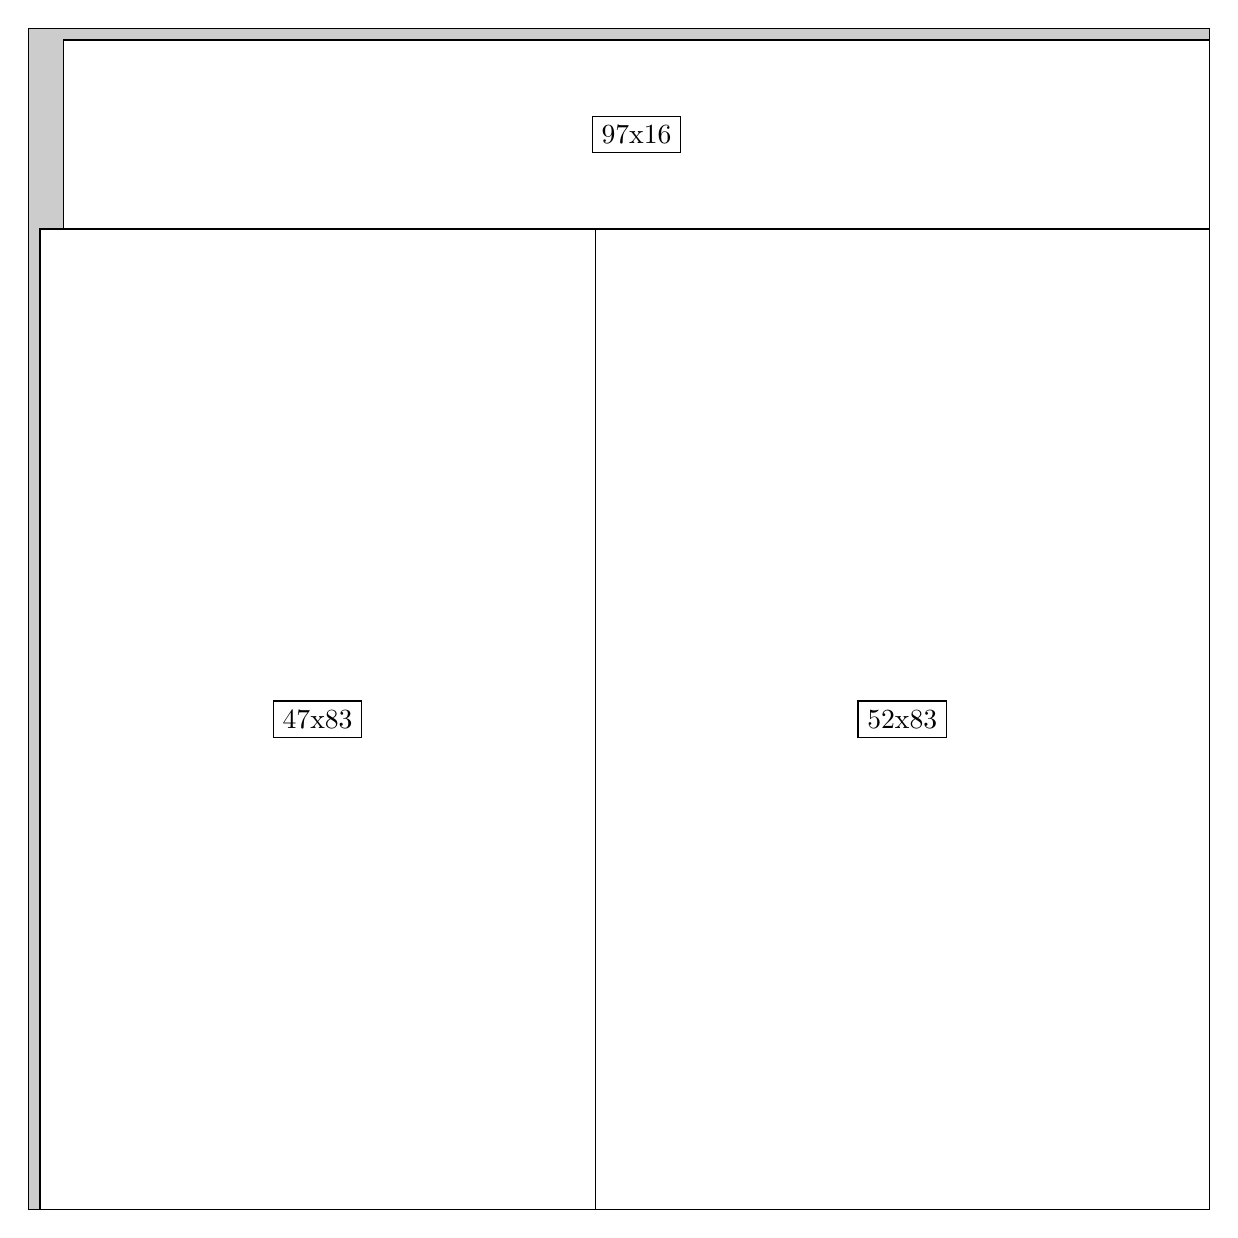
\begin{tikzpicture}[shorten >=1pt,scale=1.0,every node/.style={scale=1.0},->]
\tikzstyle{vertex}=[circle,fill=black!25,minimum size=14pt,inner sep=0pt]
\filldraw[fill=gray!40!white, draw=black] (0,0) rectangle (15.0,15.0);
\foreach \name/\x/\y/\w/\h in {52x83/7.199999999999999/0.0/7.8/12.45,47x83/0.15/0.0/7.05/12.45,97x16/0.44999999999999996/12.45/14.549999999999999/2.4}
\filldraw[fill=white!40!white, draw=black] (\x,\y) rectangle node[draw] (\name) {\name} ++(\w,\h);
\end{tikzpicture}


w =52 , h =83 , x =48 , y =0 , v =4316
\par
w =47 , h =83 , x =1 , y =0 , v =3901
\par
w =97 , h =16 , x =3 , y =83 , v =1552
\par
\newpage


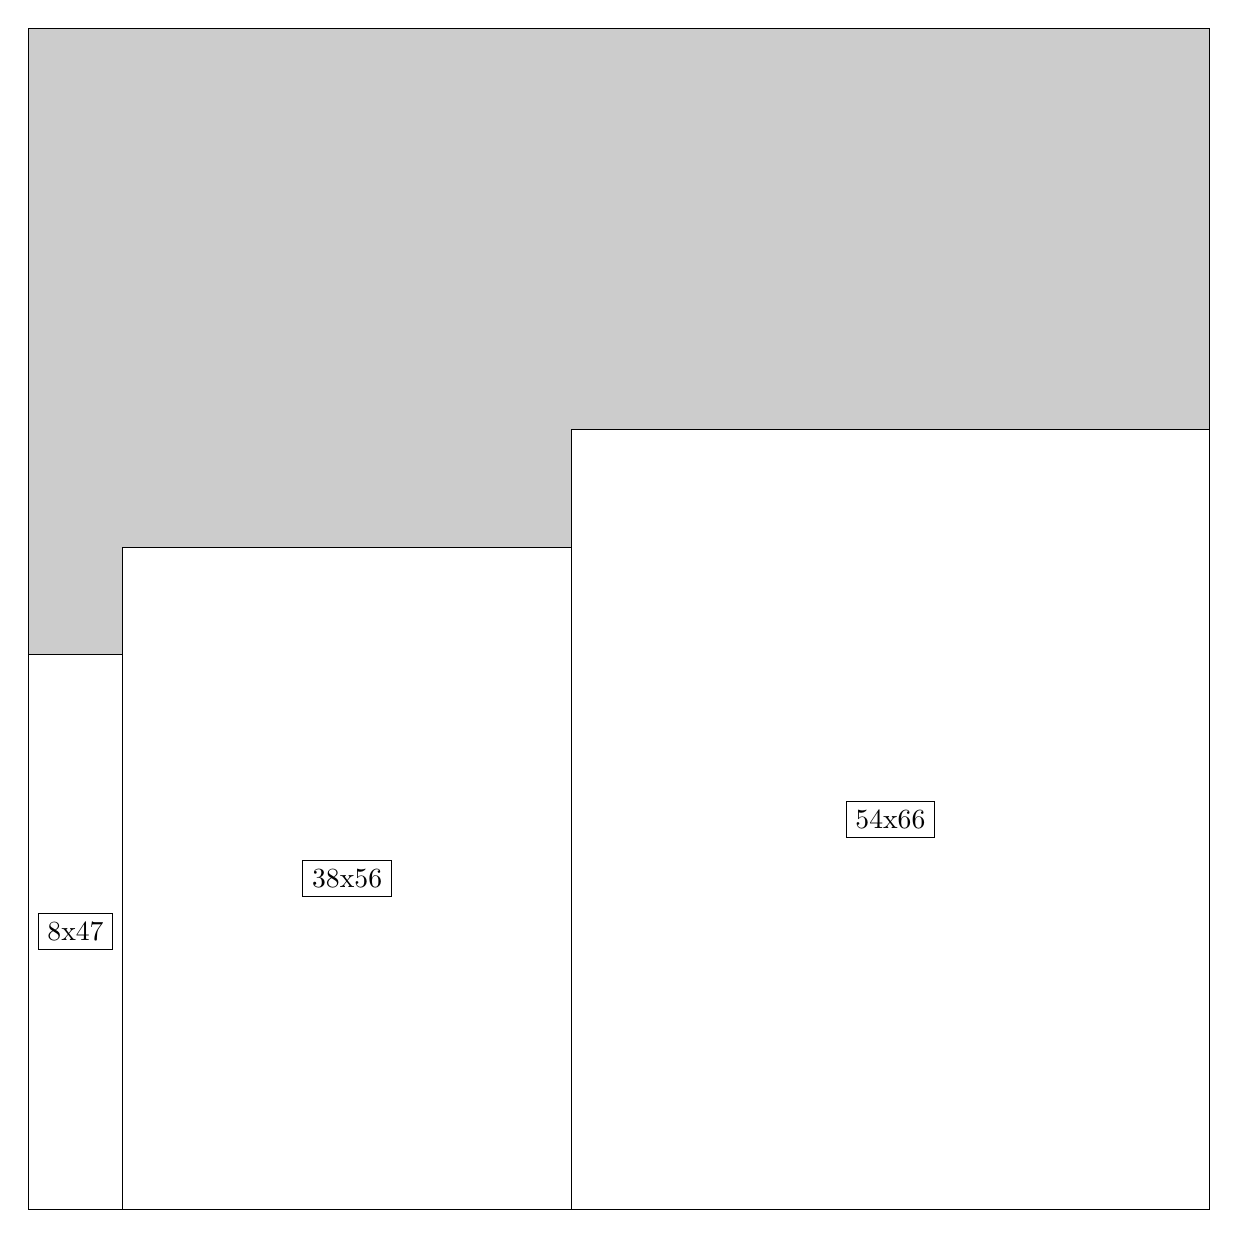
\begin{tikzpicture}[shorten >=1pt,scale=1.0,every node/.style={scale=1.0},->]
\tikzstyle{vertex}=[circle,fill=black!25,minimum size=14pt,inner sep=0pt]
\filldraw[fill=gray!40!white, draw=black] (0,0) rectangle (15.0,15.0);
\foreach \name/\x/\y/\w/\h in {54x66/6.8999999999999995/0.0/8.1/9.9,38x56/1.2/0.0/5.7/8.4,8x47/0.0/0.0/1.2/7.05}
\filldraw[fill=white!40!white, draw=black] (\x,\y) rectangle node[draw] (\name) {\name} ++(\w,\h);
\end{tikzpicture}


w =54 , h =66 , x =46 , y =0 , v =3564
\par
w =38 , h =56 , x =8 , y =0 , v =2128
\par
w =8 , h =47 , x =0 , y =0 , v =376
\par
\newpage


\end{document}